\documentclass[10pt]{scrreprt}
\usepackage[a4paper, top=30mm, left=25mm, right=25mm, bottom=30mm]{geometry}
\usepackage[utf8]{inputenc}

\usepackage[Bjornstrup]{fncychap}
\usepackage{ngerman}
\usepackage{graphicx}
\usepackage{epstopdf}
\usepackage{etoolbox}
\usepackage{enumitem}
\usepackage{url}
\usepackage{numprint}
\usepackage{longtable}
\usepackage{tabu}
\usepackage{caption}
 \usepackage{rotating}
\usepackage{array}
\usepackage{listings}
\usepackage{amssymb}


\makeatletter
\patchcmd{\@makechapterhead}{\vspace*{50\p@}}{\vspace*{-20\p@}}{}{}
\patchcmd{\@makeschapterhead}{\vspace*{50\p@}}{\vspace*{7\p@}}{}{}
\patchcmd{\DOTIS}{\vskip 40\p@}{\vskip -12\p@} 
\makeatother
  
\captionsetup[figure]{labelfont={sf,bf},textfont={sf}}
\deffootnotemark{[\thefootnotemark]}
\deffootnote{1.5em}{1em}{[\thefootnotemark] }
\setlength{\parindent}{0pt}
\renewcommand{\labelitemi}{ \raisebox{0.3ex}{\small$\blacktriangleright$} }
\renewcommand{\labelitemii}{ \raisebox{0.3ex}{\small$\triangleright$} }
\lstset{language=Java}

\newcommand{\sfbf}[1]{\textbf{\sffamily #1}}
\newcommand{\sfit}[1]{\textit{\sffamily #1}}
\newcommand{\W}{\sfbf{W}}
\newcommand{\ziel}[1]{{\fontsize{9.5}{11}\textsf{/#1/}}}
\newcommand{\ziellabel}{Z}
\newcommand{\muss}{\renewcommand{\labelenumi}{\textbf{\ziel{\ziellabel\numprint{\theenumi}0}}}}
\newcommand{\wunsch}{\renewcommand{\labelenumi}{\textbf{\ziel{\ziellabel\numprint{\theenumi}0W}}}}
\newcommand{\JoglEarth}{\raisebox{-1.2mm}{
\includegraphics[scale=0.33]{Logo-Text.eps}} }
\newcommand{\textref}[1]{\mbox{\raisebox{0.1ex}{\small$\rightarrow$ }\textit{#1}}}

\newenvironment{details}[1][6pt]{%
  \parskip#1 \parindent6mm \raggedright%
  \def\item{\par\ignorespaces\hangindent=5mm \hangafter1}}{%
  \par\ignorespaces} 
  

\begin{document}

\thispagestyle{empty}
\sffamily
 
\title{Entwurf}

\begin{figure}
\begin{flushright}
	
\includegraphics[scale=0.4]{uniLogo.eps}
\vspace{2.0 cm}
\end{flushright}
\end{figure}

\begin{center}
\vspace{2.0 cm}
{\LARGE SEP – Wintersemester 2013/14}

\vspace{1.0 cm}
\textbf{{\Huge Entwurf}}

\vspace{0.8 cm}
\begin{figure}[!htb]
\begin{center}
	%
\includegraphics[scale=1.0]{projektLogo.eps}
	
\includegraphics[scale=1.5]{Logo-Print.eps}
\end{center}
\end{figure}

\vspace{0.2 cm}
\textbf{{\huge OpenStreetMap: Die Welt in 3D}}

\vspace{1.5 cm}
15.11.2013

\vspace{0.5 cm}
Version: 1.1

\vspace{1.5 cm}
{\Large Projektbetreuer: Peter Barth}

\vspace{1.5 cm}
\begin{tabular}{|c|c|c|}
\hline 
\rule[-1ex]{0pt}{4ex} \textbf{Phase} & \textbf{Verantwortlicher} & \textbf{E-Mail Adresse} \\ 
\hline  \hline
\rule[-1ex]{0pt}{4ex} Pflichtenheft & Gabriele Haas & haasgab@fim.uni-passau.de \\ 
\hline  \hline
\rule[-1ex]{0pt}{4ex} Entwurf & Thomas Eder & ederthom@fim.uni-passau.de \\ 
\hline  \hline
\rule[-1ex]{0pt}{4ex} Spezifikation & Christof Blauberger & blauberg@fim.uni-passau.de \\ 
\hline  \hline
\rule[-1ex]{0pt}{4ex} Implementierung & Fabian Knorr & knorrfab@fim.uni-passau.de \\ 
\hline \hline 
\rule[-1ex]{0pt}{4ex} Testing & Constantin Wenger & wengerco@fim.uni-passau.de \\ 
\hline  \hline
\rule[-1ex]{0pt}{4ex} Präsentation & Sebastian Reichl & reichlse@fim.uni-passau.de \\ 
\hline 
\end{tabular}

\end{center}


\pagebreak
\rmfamily
\tableofcontents

\chapter{Einleitung}

\section*{Zu diesem Dokument}

Dieses Dokument stellt den Entwurf von \JoglEarth, der einzelnen Klassen und deren Interaktion vor. Dabei wurden die geforderten Funktionalitäten aus dem Pflichtenheft abgebildet.\\

Im Zuge der Erstellung dieses Dokuments erfolgte die Planung aller Komponenten mit deren zugehörigen Funktionen. Um das Programm im ganzen zu erfassen finden verschiedene Darstellungsarten Anwendung. \\

Als Überblick wird zu Beginn das Konzept der Anwendung mithilfe eines Architekturdiagramms erklärt. \\

Der \textit{Rational Software Architect} visualisiert die Interaktionen unter den Komponenten in Form von Diagrammen. Aus den Grafiken gehen einerseits die Vererbungshierachien, andererseits die angewendeten Design Patterns hervor. \\

Der innere Aufbau der Klassen, wie z.B. deren Methoden, wird anhand eines Klassendiagramms verdeutlicht. Wichtige Komponenten sind zusätzlich gesondert herausgearbeitet. \\

Um komplexere Zusammenhänge zu veranschaulichen werden detaillierte Auszüge aus der Klassenstruktur entnommen und in einzelne Sequenzdiagramme umgesetzt. Diese erläutern die interne Kommunikation und geben einen Überblick, zu welchem Zeitpunkt im Programmablauf eine oder mehrere Instanzen einer Komponente existiert. \\

Die Priorisierung der im Pflichtenheft angeführten Qualitätsbestimmungen besagt, dass Stabilität, Fehlertoleranz und effizientes Speichermanagement die Hauptmerkmale von \JoglEarth darstellen. Das Code Design wird den Anforderungen der Qualitätskriterien gerecht.\\

Um dem heutigen Standard hoher Softwarequalität sicherzustellen, fließen im gesamten Entwurfsprozess die gesetzten Gütekriterien und Qualitätsmerkmale ein.

\newpage

\section*{Zum Aufbau der Architektur}

Die Hauptaufgabe von \JoglEarth ist Laden großer Datenmengen aus dem Internet und deren Darstellung in OpenGL. Da die Anwendung jedoch gleichzeitig interaktiv bedienbar sein muss, ist es  unerlässlich hohe Lade- und Berechnungszeiten zu vermeiden. Die beiden Konzepte, die dieser Problematik begegnen, sowie weitere Design-Entscheidungen, die für das Verständnis des Programms wichtig sind, sollen hier kurz vorgestellt werden.

\subsection*{On-Demand-Rendering}

Statt die graphische Oberfläche kontinuierlich mit konstanter Bildrate zu rendern, wird das zeichnen eines neuen Frames bei Bedarf eventbasiert angestoßen. Solange keine Änderungen vorliegen, wird das Bild eingefroren. 

Desweiteren wird bei jeder Ansichtsänderung sofort neu gezeichnet, auch wenn noch nicht alle benötigten Kacheldaten vorliegen. In diesem Falle werden einheitliche Platzhalterdaten verwendet.


\subsection*{Datenquellen und Caching}

Das synchrone oder asynchrone Laden von Daten wird über die \textit{Source}-Schnittstelle abstrahiert. Sie bietet die Möglichkeit, generisch Daten über einen Schlüssel (\textit{Key}) abzufragen.\\[3mm]
Um unnötiges Neuladen zu verhindern, wird außerdem ein Caching-System implementiert. Caches, die auf verschiedene Speicher zurückgreifen, werden von \textit{RequestDistributor}en verwaltet. Diese vermitteln zwischen Caches und Quellen, sind für die Verdrängung zuständig und verhalten sich selbst wie gewöhnliche Datenquellen.

\subsection*{Geometry und Tesselatoren}
Da \JoglEarth mehrere verschiedene Arten der dreidimensionalen Darstellung bietet (Globus und Kartenebene), wird eine weitere Abstraktionsschicht eingeführt.

Räumliche Berechnungen, die vom Ansichtsmodus abhängig sind werden von Implementierungen des \textit{Geometry}-Interfaces erledigt; Das erzeugen der OpenGL-Rohdaten für das 3D-Modell geschieht über Konzept des \textit{Tesselators}.


\chapter{UML-Klassendiagramme}

\section{Packages}
Folgende Abbildung gibt einen Überblick über die gesamten Packages.\\

\begin{figure}[!htb]
\begin{center}
	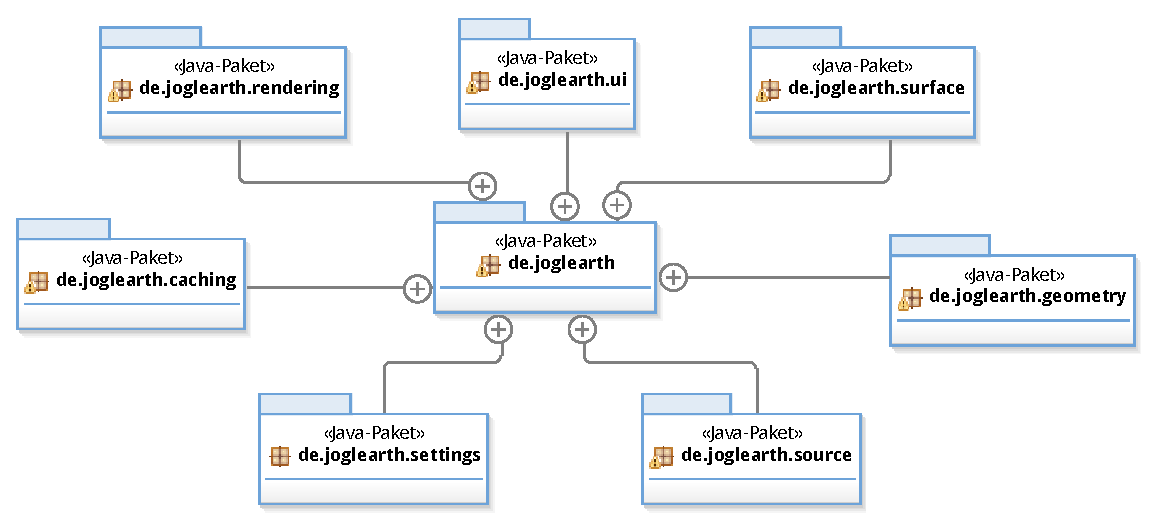
\includegraphics[scale=0.55]{Pakete.eps}
\end{center}
\end{figure}

\begin{itemize}
\item \textbf{\sffamily de.joglearth} ist der Container für alle anderen Packages und enthält die Hauptklasse \textit{JoglEarth}.
\begin{itemize}
\item \textbf{\sffamily de.joglearth.caching} stellt die Caching-Funktionalität bereit.
\item \textbf{\sffamily de.joglearth.geometry} beinhaltet Klassen für die geometrischen Ansichts- und Sichtbarkeitsberechnungen sowie die mathematische Beschreibung der Darstellungsmodelle.
\item \textbf{\sffamily de.joglearth.rendering} enthält Klassen zur Umsetzung des mathematischen Modells in eine 3D-Darstellung mit OpenGL.
\item \textbf{\sffamily de.joglearth.settings} ist für die Verwaltung von Benutzereinstellungen und Benachrichtigung bei deren Änderung zuständig.
\item \textbf{\sffamily de.joglearth.source} beinhaltet Klassen zum synchronen und asynchronen Zugriff auf externe Daten.
\item \textbf{\sffamily de.joglearth.surface} enthält Komponenten zur Verwaltung von Objekten und Eigenschaften der Erdoberfläche wie dem Kartenmaterial, dem Höhenprofil und der Overlays.
\item \textbf{\sffamily de.joglearth.ui} fasst Klassen der grafischen Benutzeroberfläche zusammen.
\end{itemize}
\end{itemize}

\newpage

\section{Interfaces, Klassen und Enumerations}

Im Folgenden werden UML-Diagramme für die Elemente der einzelnen Packages gezeigt.

Eine vollständige Ansicht der Klassenstruktur findet sich im Anhang unter Abbildung 9.4.

\vspace{2mm}

\begin{figure}[!htb]
	\centering
		\begin{minipage}[c]{3cm}
        \centering
			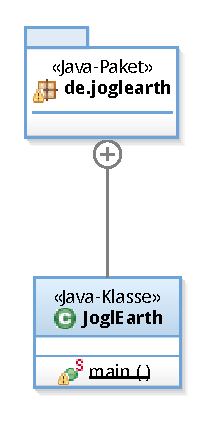
\includegraphics[scale=0.55]{de_joglearth.eps}
        \end{minipage}
        \hspace{2cm}
        \begin{minipage}[c]{6cm}
        \centering
			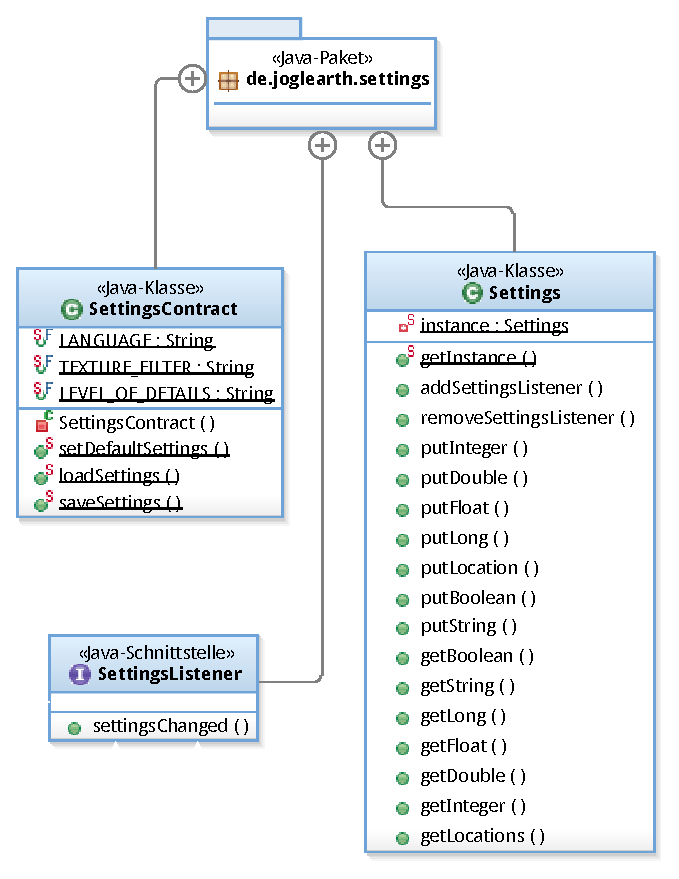
\includegraphics[scale=0.55]{de_joglearth_settings.eps}
        \end{minipage}
        \caption{Packages de.joglearth und de.joglearth.settings}
\end{figure}

\vspace{2mm}

\begin{figure}[!htb]
\begin{center}
	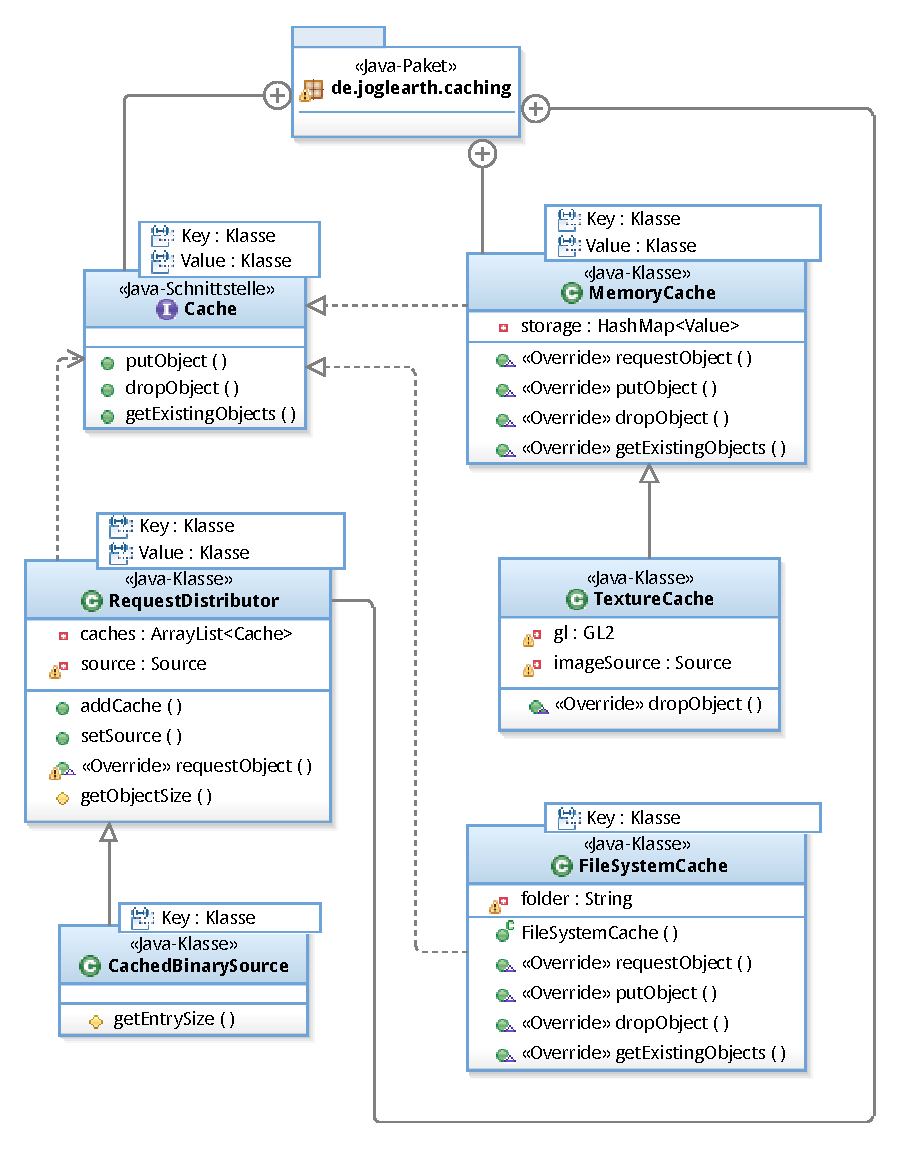
\includegraphics[scale=0.55]{de_joglearth_caching.eps}
\end{center}
\caption{Das Package de.joglearth.caching}
\end{figure}


\begin{figure}[!htb]
\begin{center}
	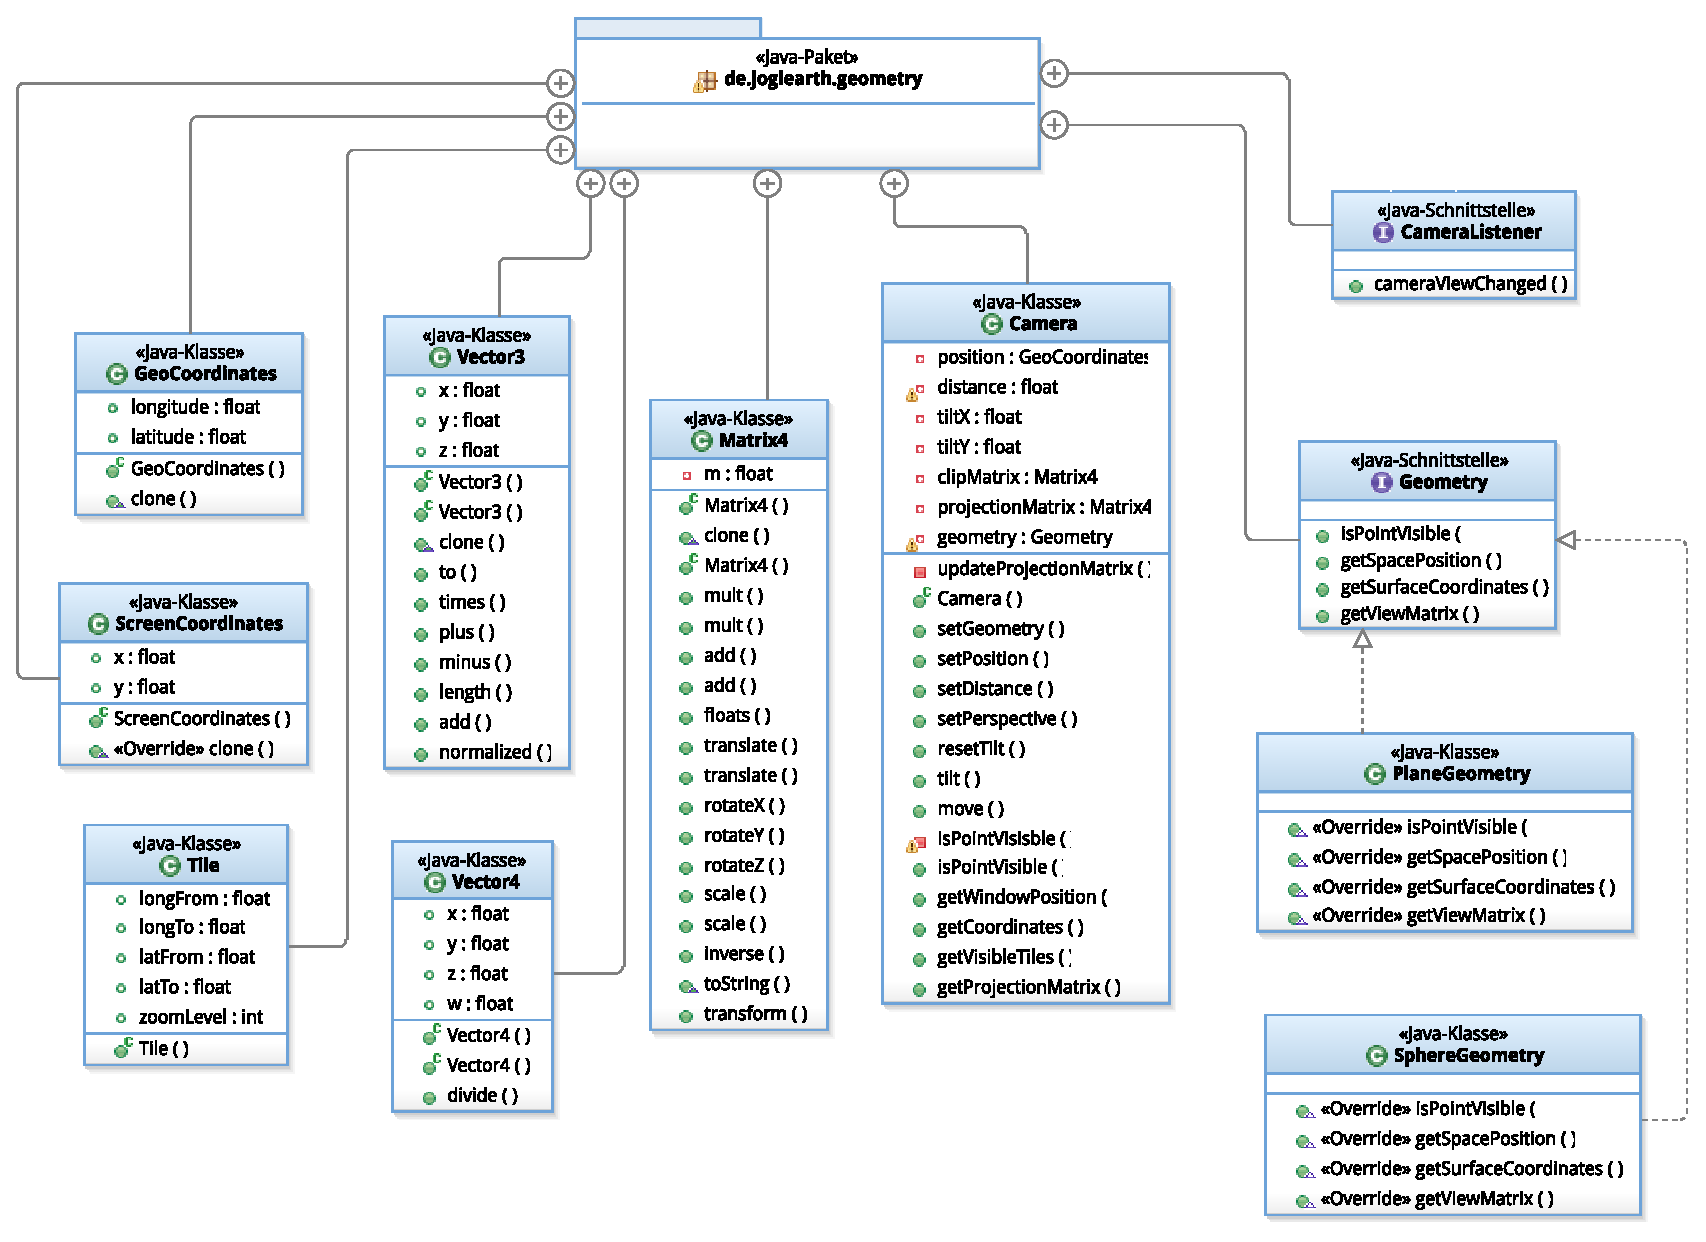
\includegraphics[scale=0.55]{de_joglearth_geometry.eps}
\end{center}
\caption{Das Package de.joglearth.geometry}
\end{figure}

\begin{figure}[!htb]
\begin{center}
	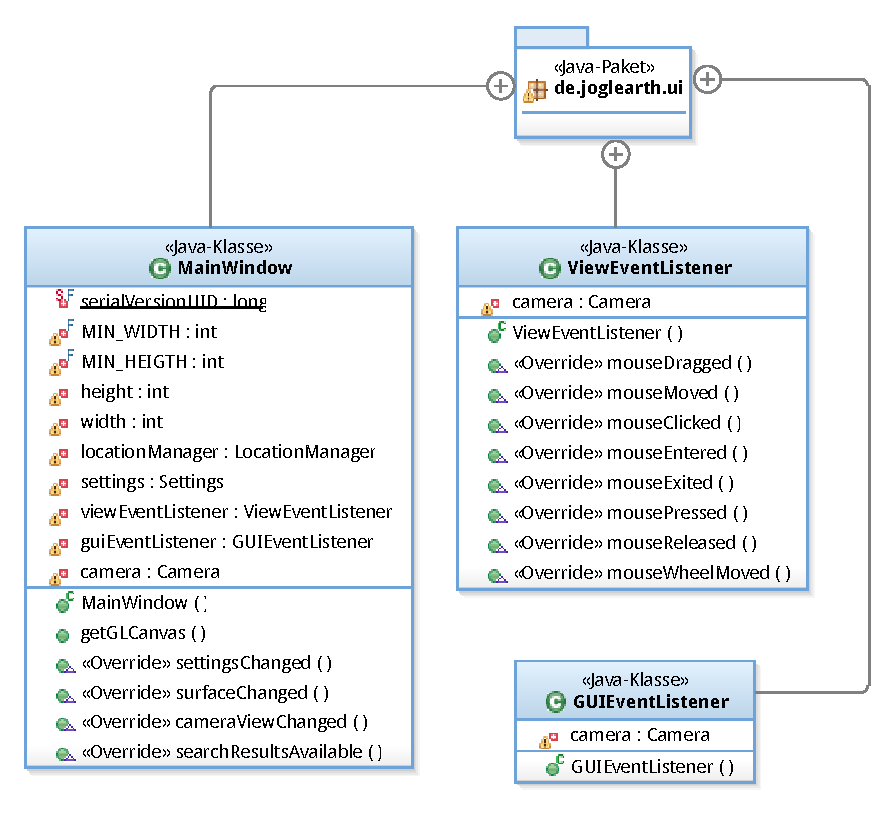
\includegraphics[scale=0.55]{de_joglearth_ui.eps}
\end{center}
\caption{Das Package de.joglearth.ui}
\end{figure}

\begin{figure}[!htb]
\begin{center}
	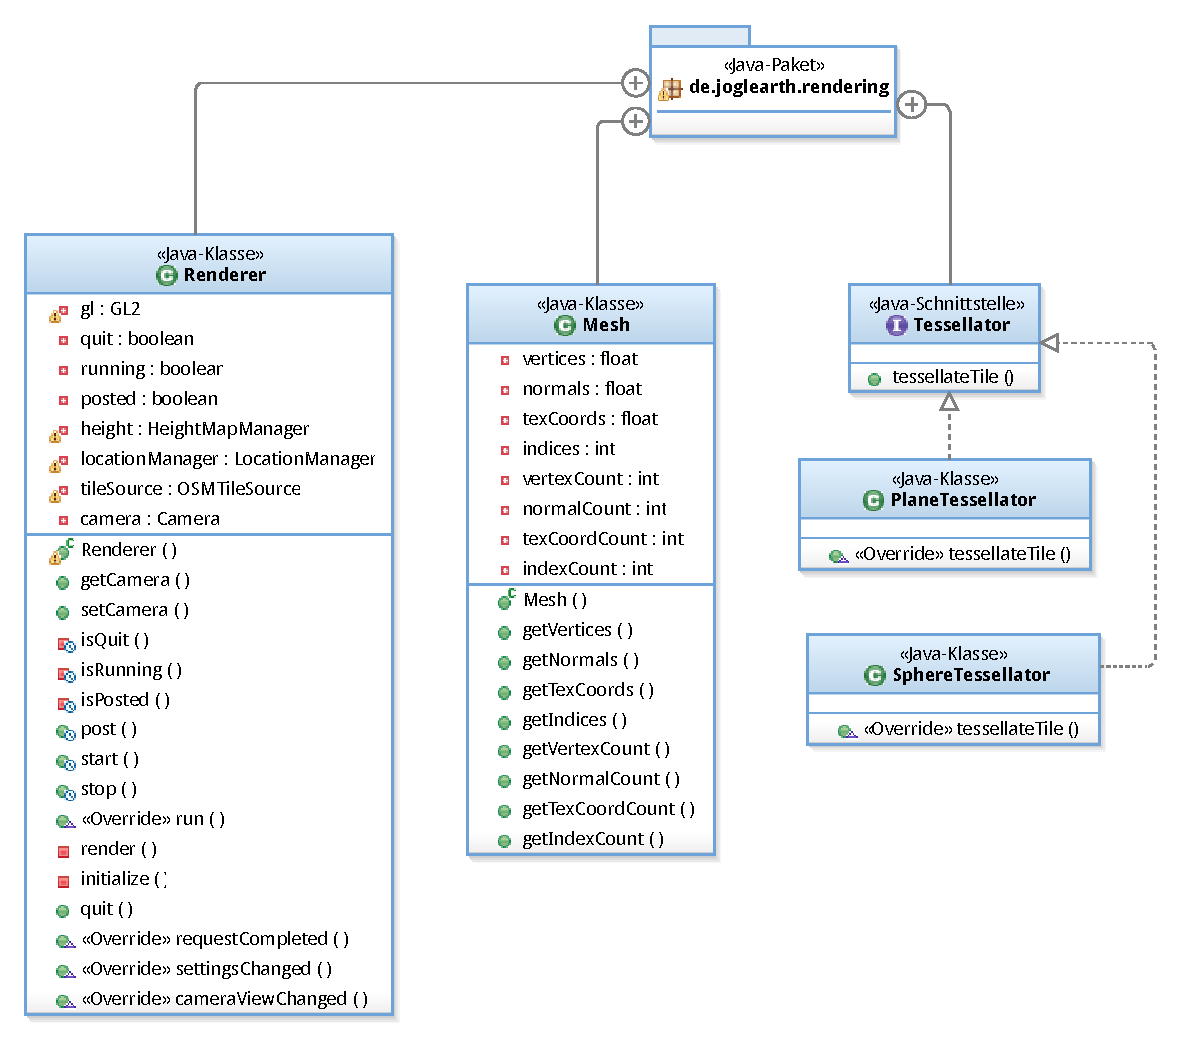
\includegraphics[scale=0.55]{de_joglearth_rendering.eps}
\end{center}
\caption{Das Package de.joglearth.rendering}
\end{figure}

\begin{figure}[!htb]
\begin{center}
	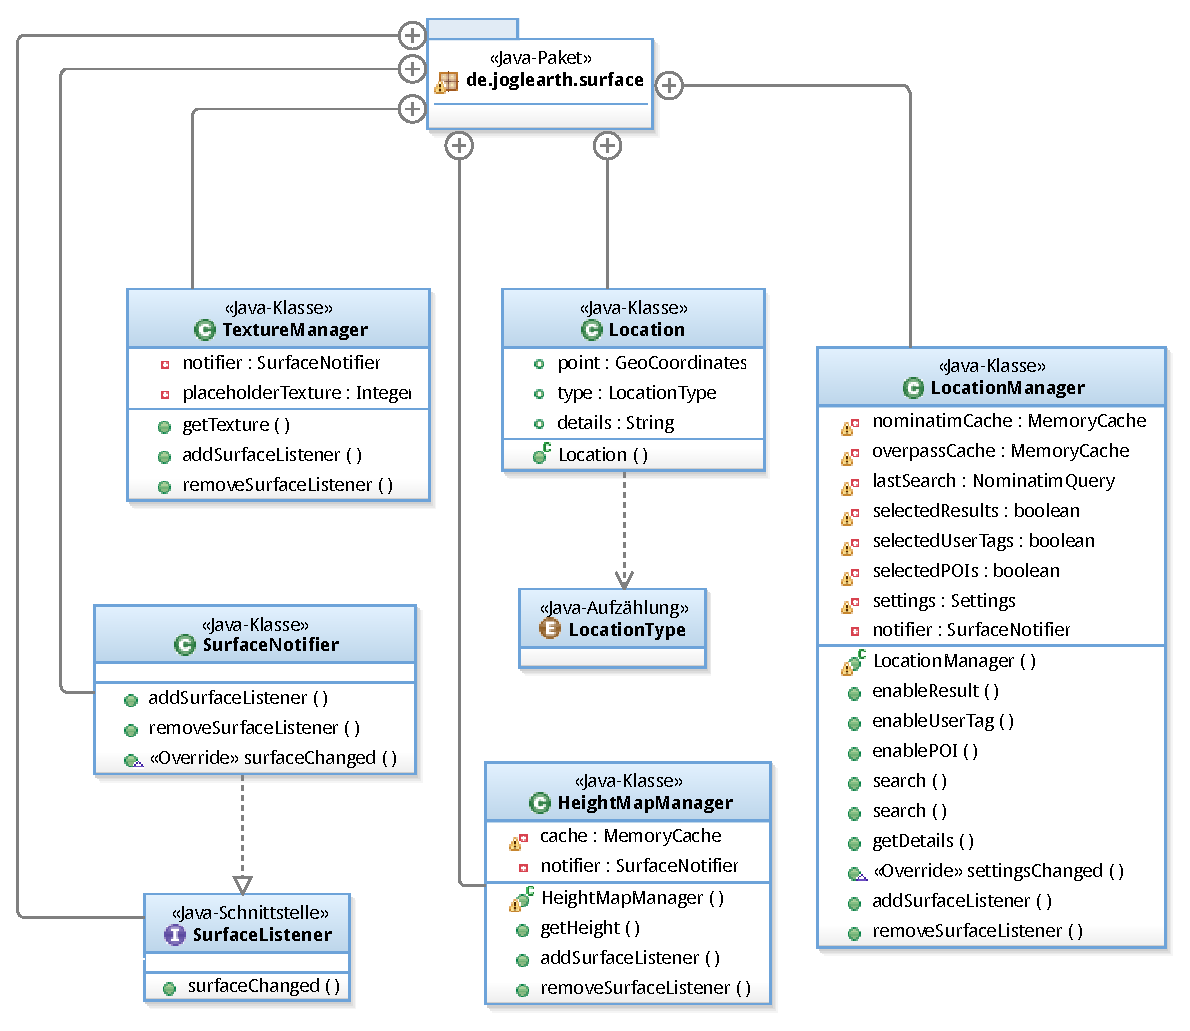
\includegraphics[scale=0.55]{de_joglearth_surface.eps}
\end{center}
\caption{Das Package de.joglearth.surface}
\end{figure}


\begin{figure}[!htb]
\begin{center}
	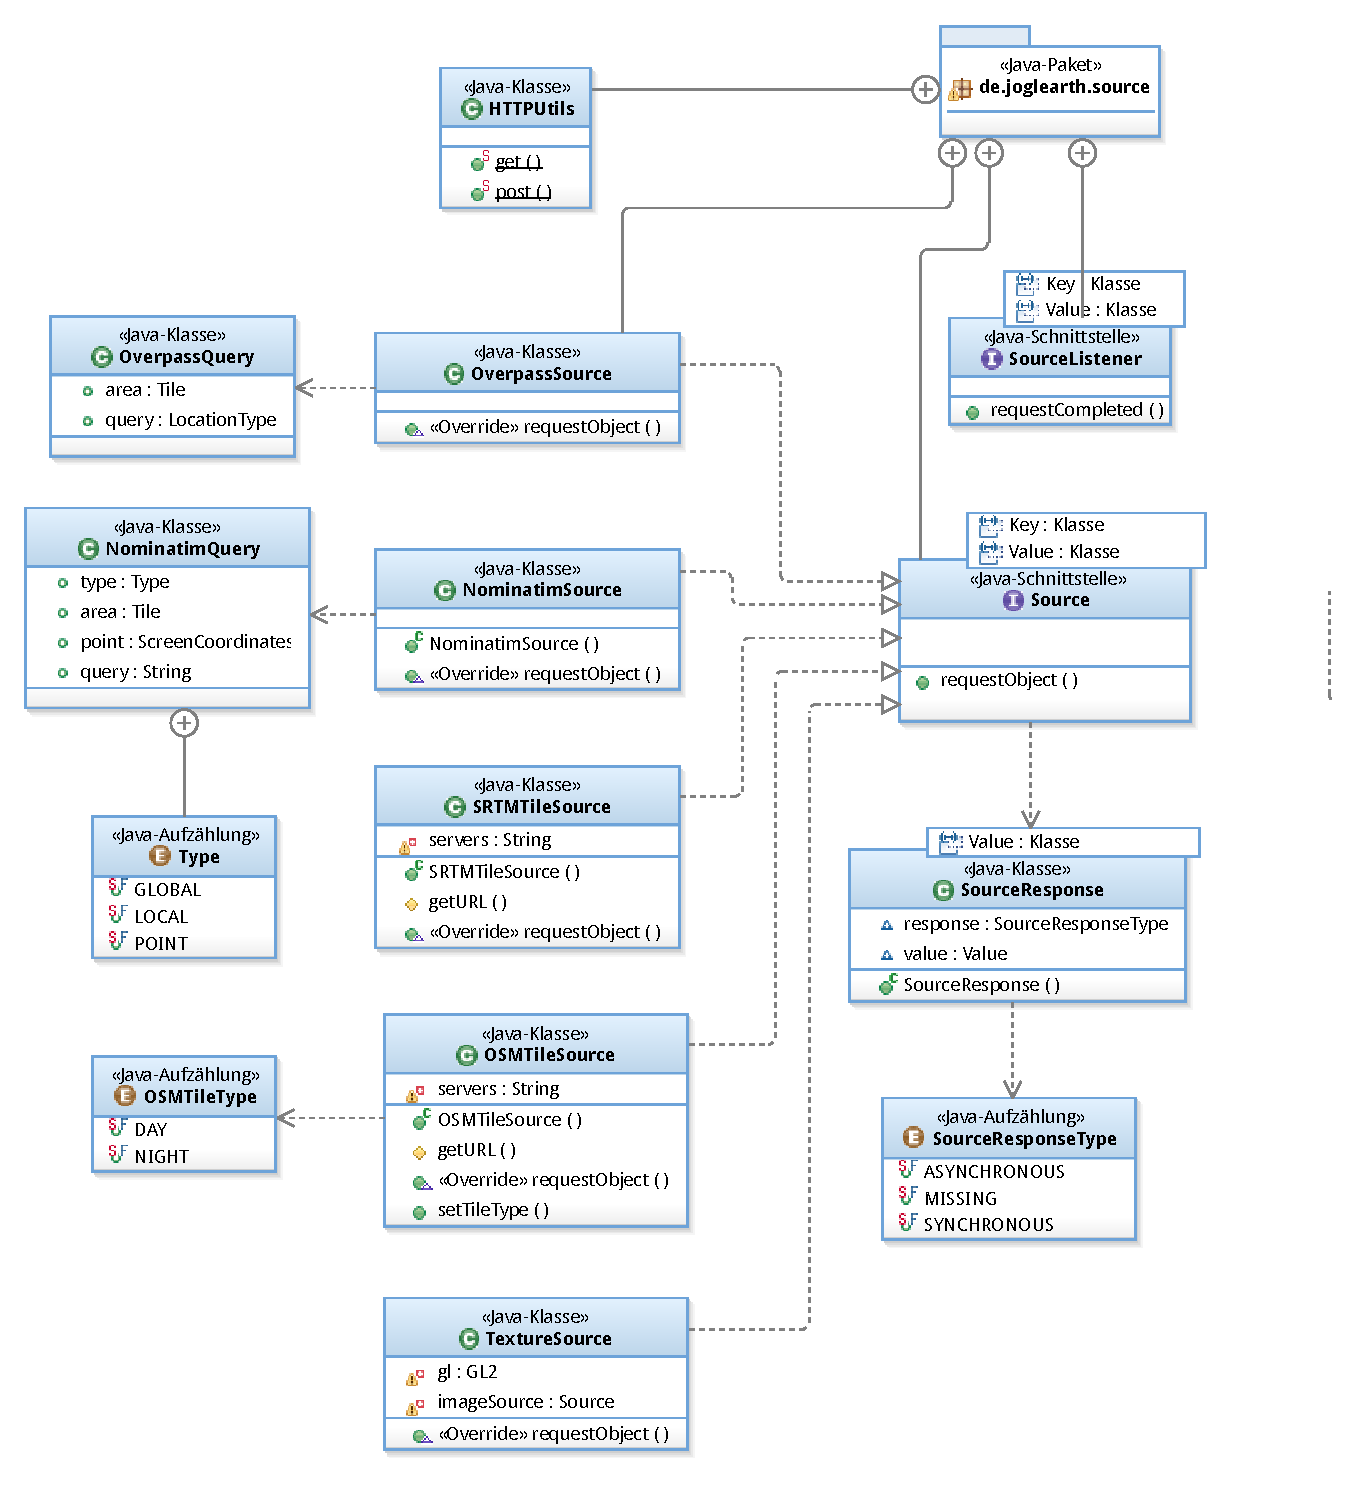
\includegraphics[scale=0.55]{de_joglearth_source.eps}
\end{center}
\caption{Das Package de.joglearth.source}
\end{figure}



\chapter{Beschreibung der Interfaces}

\section{Package de.joglearth.caching}
\subsection*{Cache}
\begin{lstlisting}
interface Cache<Key, Value>
extends Source<Key, Value>
\end{lstlisting}
Bildet die Schnittstelle für einen Cache, der Methoden zum Hinzufügen, Abfragen und Löschen von Daten bietet. Die Verwaltung der Größenbeschränkungen und die Implementierung der Verdrängungsstrategie ist Sache des \textit{RequestDistributors}.\\
\subsubsection*{Methoden (Auszug)}
\begin{itemize}
\item \texttt{putObject()} legt ein Objekt, identifiziert über einen \textit{Key}, in den Cache. Dies kann zur Folge haben, das ein bereits existierendes Objekt mit diesem Schlüssel überschrieben wird. Eine Verdrängung findet niFcht statt, diese ist Aufgabe des übergeordneten \textit{RequestDistributors}.
\item \texttt{dropObject()} entfernt ein Objekt über seinen \textit{Key} aus dem Cache.
\item \texttt{requestObject()} fordert ein Objekt an. Die Schnittstelle entspricht der von \textit{Source}.
\end{itemize}
\vspace{5mm}


\section{Package de.joglearth.geometry}
\subsection*{Geometry}
\begin{lstlisting}
interface Geometry
\end{lstlisting}
Abstrahiert den Teil der Sichtbarkeits- und Positionsberechnungen, der vom gewählten Oberflächenmodell (Globus oder Kartenebene) abhängt. Die Kamera besitzt ein solches Geometry-Objekt, um sich dem Ansichtsmodus entsprechend zu verhalten.\\

\vspace{5mm}
\subsection*{CameraListener}
\begin{lstlisting}
interface CameraListener
\end{lstlisting}
Interface für Klassen, die Events beim Ändern von Kameraposition und -einstellungen entgegennehmen können.\\

\pagebreak
\vspace{5mm}
\section{Package de.joglearth.rendering}
\subsection*{Tessellator}
\begin{lstlisting}
interface Tessellator
\end{lstlisting}
Bietet eine gemeinsame Schnittstelle für das Erzeugen von dreidimensionalen Kacheln verschiedener geometrischer Modelle. Sie wird vom Renderer benutzt, um den Ansichtseinstellungen gemäß ein dreidimensionales Modell zu generieren.\\
\subsubsection*{Methoden (Auszug)}
\begin{itemize}
\item \texttt{tesselateTile()} erzeugt aus den geometrischen Angaben eines \textit{Tiles} und der Heightmap einen \textit{Mesh}, der zum Zeichnen an OpenGL übergeben werden kann.
\end{itemize}


\vspace{5mm}
\section{Package de.joglearth.settings}
\subsection*{SettingsListener}
\begin{lstlisting}
interface SettingsListener
\end{lstlisting}
Eine Implementierung des \textit{SettingsListeners} kann über Änderungen der \textit{Settings} benachrichtigt werden. Das Interface ist damit intergraler Bestandteil des Settings-Mechanismus, der Benutzereinstellungen an die zuständigen Komponenten vermittelt.\\


\vspace{5mm}
\section{Package de.joglearth.source}
\subsection*{Source}
\begin{lstlisting}
interface Source<Key, Value>
\end{lstlisting}
Eine \textit{Source} ist eine Datenquelle, die in der Lage ist, über einen \texttt{Key} identifizierte Objekte synchron oder asynchron zu beschaffen. Sowohl die ursprünglichen HTTP-Clients als auch Caches und cacheverwaltende Klassen verhalten sich gemäß dieser Schnittstelle.\\
\subsubsection*{Methoden (Auszug)}
\begin{itemize}
\item \texttt{requestObject()} führt eine Anfrage nach einem Objekt über seinen \textit{Key} durch. Die Methode gibt eine \textit{SourceResponse}-Struktur zurück, die das synchron beschaffte Objekt enthält, falls dies ohne nennenswerten Zeitverlust möglich war, oder einen Indikator dafür, dass die Antwort asynchron nachgeliefert wird bzw. nicht beschafft werden kann.
\end{itemize}

\vspace{5mm}
\subsection*{SourceListener}
\begin{lstlisting}
interface SourceListener<Key, Value>
\end{lstlisting}
Eine Implementierung dieses Interfaces kann asynchrone Antworten zur \textit{requestObject()}-Anfrage einer \textit{Source} entgegen nehmen.\\

\pagebreak
\section{Package de.joglearth.surface}
\subsection*{SurfaceListener}
\begin{lstlisting}
interface SurfaceListener
\end{lstlisting}
Klassen, die dieses Interface implementieren, können über Änderungen in der Darstellung einzelner Kartenkacheln benachrichtigt werden.\\
\subsubsection*{Methoden (Auszug)}
\begin{itemize}
\item \texttt{surfaceChanged()} ist ein Callback, dessen Aufruf anzeigt, dass sich die Oberfläche einer bestimmten Kachel auf irgendeine Weise geändert hat. Dies kann beispielsweise durch verspätetes Nachladen einer Textur oder das hinzufügen einer Benutzermarkierung geschehen.
\end{itemize}


\vspace{5mm}
\subsection*{LocationListener}
\begin{lstlisting}
interface LocationListener
\end{lstlisting}
Eine Implementierung dieses Interfaces nimmt asynchrone Antworten des \textit{LocationManagers}, wie geladene Suchergebnisse, entgegen.\\




\chapter{Beschreibung der Klassen}
\section{Package de.joglearth}
\subsection*{JoglEarth}
\begin{lstlisting}
final class JoglEarth
\end{lstlisting}
Dies ist die Hauptklasse des Programms.\\
\subsubsection*{Methoden (Auszug)}
\begin{itemize}\item\texttt{main()} Startet die Anwendung.
\end{itemize}


\vspace{5mm}
\section{Package de.joglearth.caching}
\subsection*{RequestDistributor}
\begin{lstlisting}
class RequestDistributor<Key, Value>
implements Source<Key, Value>
\end{lstlisting}
Lädt Daten aus einer \textit{Source}, verwaltet diese in Caches und ist für deren Verdrängung verantwortlich.\\
Ein \textit{RequestDistributor} hat Zugriff auf genau eine ursprüngliche \textit{Source}, von der alle Datenelemente stammen, sowie auf eine beliebige Anzahl an Caches, die eine Cachehierarchie bilden.\\
Für jeden Cache lässt sich eine Maximalgröße in \textit{Einheiten} festlegen. Für einen (reinen) \textit{RequestDistributor} ist jeder Eintrag eine Einheit groß, d.h. die Größenbeschränkung bezieht sich auf die Anzahl der Elemente.\\
\subsubsection*{Methoden (Auszug)}
\begin{itemize}
\item \texttt{requestObject()} verhält sich wie \texttt{Source.requestObject()}. Anfragen werden bevorzugt über die Caches beantwortet. Ist das nicht mögilch, so werden die Daten über die \textit{Source} nachgeladen und das Ergebnis in den ersten Cache der Hierarchie gelegt. Überschreitet er seine zulässige Maximalgröße, werden bestehende Einträge (wenn möglich in den nachfolgenden Cache) verdrängt. 
\end{itemize}
\vspace{5mm}
\subsection*{BinaryRequestDistributor}
\begin{lstlisting}
class BinaryRequestDistributor<Key>
extends RequestDistributor<Key, byte[]>
\end{lstlisting}
Erweitert den \textit{RequestDistributor} um die Möglichkeit den Cache nach Größe statt nach Anzahl der Einträge zu begrenzen. Eine \textit{Einheit} (s. \textit{RequestDistributor}) bezeichnet in dieser Klasse ein Byte im Datenobjekt.
\pagebreak
\subsection*{FileSystemCache}
\begin{lstlisting}
class FileSystemCache<Key>
implements Cache<Key, byte[]>
\end{lstlisting}
Ein \textit{FileSystemCache} speichert Daten im Dateisystem zwischen. Da Dateien Byteströme sind, kann er ausschließlich Byte-Arrays als Wertdaten aufnehmen.\\

\vspace{5mm}
\subsection*{MemoryCache}
\begin{lstlisting}
class MemoryCache<Key, Value>
implements Cache<Key, Value>
\end{lstlisting}
Ein \textit{MemoryCache} speichert Daten im Arbeitsspeicher ähnlich einer \textit{HashMap} zwischen. Er ist für jeden Wertdatentyp geeignet.\\

\vspace{5mm}
\subsection*{TextureCache}
\begin{lstlisting}
class TextureCache
extends MemoryCache<Tile, Integer>
\end{lstlisting}
Ein \textit{TextureCache} verwaltet in OpenGL geladene Texturen.

Wegen seiner Eigenschaft als Cache kann er nur bereits bestehende Texturen verwalten und diese verdrängen, was zum Löschen der Textur aus dem Grafikspeicher führt. 

Da Texturen in der OpenGL-API über \textit{int}s identifiziert werden, ist der Wertdatentyp ebenfalls ein Integer.\\


\vspace{5mm}
\section{Package de.joglearth.geometry}
\subsection*{Camera}
\begin{lstlisting}
class Camera
\end{lstlisting}
Berechnet die Projektionsmatrix für den Rendervorgang, bestimmt die Sichtbarkeit von 3D-Objekten im Ansichtsfenster und rechnet zwischen Bildschirm- und Raumkoordinaten um.\\
Enthält eine Methode zum Setzen einer \textit{Geometry} für die Unterscheidung zwischen sphärischen und planaren Bewegungsberechnungen.\\
\subsubsection*{Methoden (Auszug)}
\begin{itemize}
\item \texttt{getVisibleTiles()} bestimmt die Menge aller momentan sichtbaren Kacheln. Die Größe (der Winkelabstand zwischen den Kanten) wird dabei so bestimmt, dass ihre Anzahl unabhängig vom Zoomlevel und der Position in einem festgelegten Bereich liegt.
\item \texttt{getProjectionMatrix()} berechnet die \textit{Projektionsmatrix}, die OpenGL zum Rendern des Modells übergeben wird. Durch die Tatsache, dass die Sicht bereits vollständig durch diese Struktur beschrieben wird, ermöglicht es, dass die \textit{Tesselatoren} das 3D-Modell unabhängig von der Drehung oder Verschiebung des Globus bzw. der Ebene berechnen können.
\end{itemize}

\vspace{2mm}
\subsection*{GeoCoordinates}
\begin{lstlisting}
class GeoCoordinates
implements Cloneable
\end{lstlisting}
Speichert Längen- und Breitengrad eines Punktes auf der Erdoberfläche.

\pagebreak

\subsection*{Matrix4}
\begin{lstlisting}
class Matrix4
implements Cloneable
\end{lstlisting}
Hält eine 4x4-Matrix, die Operationen zum Rotieren, Verschieben und Skalieren, sowie eine Funktion zum transformieren eines dreidimensionalen Vektors anbietet. Sie wird zum von der Kamera intern zum Bestimmen der Projektionsmatrix und der Sichtbarkeit von Objekten verwendet.\\
\subsubsection*{Methoden (Auszug)}
\begin{itemize}
\item \texttt{transform()} Transformiert einen dreidimensionalen Vektor im Modellbreich in einen vierdimensionalen homogenen Vektor im Bildbereich. Der Punkt wird dadurch von seiner ursprünglichen Position so verschoben und perspektivisch verzerrt, wie ihn der Betrachter am Kameraursprung sehen würde.

Mit Hilfe dieser Methode kann unter anderem bestimmt werden, an welcher Stelle des Bildes zweidimensionale Overlays zum liegen kommen.
\end{itemize}

\vspace{5mm}
\subsection*{PlaneGeometry}
\begin{lstlisting}
class PlaneGeometry
implements Geometry
\end{lstlisting}
Implementiert das \textit{Geometry}-Interface für räumliche Berechnungen auf einer Ebene.\\

\vspace{5mm}
\subsection*{ScreenCoordinates}
\begin{lstlisting}
class ScreenCoordinates
implements Cloneable
\end{lstlisting}
Stellt einen Punkt auf der Bildschirmebene in relativen Koodrinaten zwischen 0 und 1 dar.\\

\vspace{5mm}
\subsection*{SphereGeometry}
\begin{lstlisting}
class SphereGeometry
implements Geometry
\end{lstlisting}
Implementiert das \textit{Geometry}-Interface für räumliche Berechnungen auf der Kugeloberfläche.\\

\vspace{5mm}
\subsection*{Tile}
\begin{lstlisting}
class Tile 
implements Cloneable
\end{lstlisting}
Speichert Längen- und Breitengradgrenzen sowie das Zoomlevel einer Kachel.

Darüber lassen sich Kartenkacheln von OpenStreetMap identifizieren, Bereiche für eine lokale Suche mit Nominatim vorgeben, und Anweisungen an den \textit{Tesselator} formulieren.\\

\pagebreak
\subsection*{Vector3}
\begin{lstlisting}
class Vector3
implements Cloneable
\end{lstlisting}
Ein dreidimensionaler Vektor, der für Raumkoordinaten verwendet wird.\\

\vspace{5mm}
\subsection*{Vector4}
\begin{lstlisting}
class Vector4
implements Cloneable
\end{lstlisting}
Ein vierdimensionaler Vektor für homogene Koordinaten. Diese Klasse findet Verwendung, wenn zwischen Perspektiven umgerechnet werden soll (s. \texttt{Matrix4.transform()}).\\
\subsubsection*{Methoden (Auszug)}
\begin{itemize}
\item \texttt{divide()} wandelt den vier- in einen dreidimensionalen Vektor um, der perspektivisch vergrößert oder verkleinert wurde.
\end{itemize}





\vspace{5mm}
\section{Package de.joglearth.rendering}
\subsection*{Mesh}
\begin{lstlisting}
class Mesh
\end{lstlisting}
Speichert Rohdaten eines 3D-Modells wie seine Vertices, Normalen, und Texturkoordinaten. Meshes werden von \textit{Tessellatoren} generiert und vom \textit{Renderer} an OpenGL übergeben.\\

\vspace{5mm}
\subsection*{PlaneTessellator}
\begin{lstlisting}
class PlaneTessellator
implements Tessellator
\end{lstlisting}
Erzeugt Kachelmeshes in der Ebene.\\

\vspace{5mm}
\subsection*{Renderer}
\begin{lstlisting}
class Renderer
implements SourceListener<Tile, Integer>, Runnable, CameraListener,
           SettingsListener
\end{lstlisting}
Ist für das Zeichnen einzelner Frames und die zeitliche Steuerung während der Animationen verantwortlich. Er rendert entweder Einzelbilder als Reaktion auf eine Aktualisierung der Szene durch den \textit{SourceListener}, \textit{CameraListener} oder \textit{SettingsListener}, oder eine kontinuierliche Bildfolge während Animationsvorgängen.\\
\subsubsection*{Methoden (Auszug)}
\begin{itemize}
\item \texttt{start()} startet einen kontinuierlichen Rendervorgang mit konstanter Bildrate.
\item \texttt{stop()} beendet das kontinuierliche Rendern.
\item \texttt{post()} benachrichtigt den Renderer, dass noch mindestens ein Frame gezeichnet werden muss. Mehrere dieser Aufrufe können vom Renderer zusammengefasst, oder gar ignoriert werden falls bereits eine kontinuierliche Bildaktualisierung läuft.
\end{itemize}
Alle drei vorgestellten Methoden arbeiten asynchron, d.h. sie stoßen den Rendervorgang in einem Hintergrundthread an.

\vspace{5mm}
\subsection*{SphereTessellator}
\begin{lstlisting}
class SphereTessellator
implements Tessellator
\end{lstlisting}
Generiert Kachelmeshes auf der Globusoberfläche.\\




\vspace{5mm}
\section{Package de.joglearth.settings}
\subsection*{Settings}
\begin{lstlisting}
class Settings
\end{lstlisting}
Verwaltet alle erforderlichen Einstellungen sowie die vom Benutzer markierten Punkte aus der Datei \texttt{settings.xml}. Die Einstellungen werden gekapselt und anderen Klassen zugänglich gemacht, außerdem können sich andere Klassen als Beobachter (\textit{Observer}) registrieren um über Einstellungsänderungen benachrichtigt zu werden.\\
\subsubsection*{Methoden (Beispiele)}
\begin{itemize}
\item \texttt{getInteger()} liest eine Ganzzahl, die über einen \textit{Property}-Namen identifiziert wird.
\item \texttt{putInteger()} schreibt eine Ganzzahl.
\item \texttt{getInstance()} gibt die globale Settings-Instanz zurück (siehe Singleton-Pattern)
\end{itemize}

\vspace{5mm}
\subsection*{SettingsContract}
\begin{lstlisting}
final class SettingsContract
\end{lstlisting}
Enthält die möglichen \textit{Property}-Namen der Settings in dieser Anwendung und ist für das Laden und Speichern in die XML-Datei \texttt{settings.xml} verantwortlich.\\
\subsubsection*{Methoden (Auszug)}
\begin{itemize}
\item \texttt{loadSettings()} lädt die Settings aus der Einstellungsdatei.
\item \texttt{setDefaultSettings()} speichert sie.
\end{itemize}



\pagebreak
\section{Package de.joglearth.source}
\subsection*{HTTPUtils}
\begin{lstlisting}
final class HTTPUtils
\end{lstlisting}
Stellt statische Funktionen für einfache GET- und POST- Abfragen via HTTP zur Verfügung.\\
\subsubsection*{Methoden (Auszug)}
\begin{itemize}
\item \texttt{get()} führt eine (synchrone) HTTP-GET-Anfrage auf einem Server durch.
\item \texttt{post()} führt eine (synchrone) HTTP-POST-Anfrage durch, der zusätzliche Daten mitgegeben werden können.
\end{itemize}

\vspace{5mm}
\subsection*{NominatimQuery}
\begin{lstlisting}
class NominatimQuery
\end{lstlisting}
Drückt eine Suchanfrage an Nominatim aus. Dies kann die Suche nach Details zu einem bestimmten Punkt oder nach einem Ort sein.\\

\vspace{5mm}
\subsection*{NominatimSource}
\begin{lstlisting}
class NominatimSource
implements Source<NominatimQuery, Location[]>
\end{lstlisting}
\textit{NominatimSource} beschafft Antworten auf Suchanfragen nach Orten und Punktinformationen (\textit{NominatemQuery}) und bereitet sie für den \textit{LocationManager} auf. Dabei greift sie auf \textit{HTTPUtils} zu.\\

\vspace{5mm}
\subsection*{OSMTileSource}
\begin{lstlisting}
class OSMTileSource
implements Source<Tile, byte[]>
\end{lstlisting}
Die \textit{OSMTileSource} lädt anhand von Koordinaten (u. U. komprimierte) Kacheltexturen per HTTP von OpenStreetMap-Servern. Dabei macht sie von \textit{HTTPUtils} Gebrauch.\\

\vspace{5mm}
\subsection*{OverpassQuery}
\begin{lstlisting}
class OverpassQuery
\end{lstlisting}
Drückt eine Suchanfrage an die OverpassAPI aus. Eine solche Suche liefert für gewöhnlich POIs und Städtenamen im Sichtfeld zurück. Die Anfrage enthält dazu die zu durchsuchende Umgebung.\\

\pagebreak
\subsection*{OverpassSource}
\begin{lstlisting}
class OverpassSource
implements Source<OverpassQuery, Location[]>
\end{lstlisting}
\textit{OverpassSource} beschafft die Details lokaler POIs und Städtenamen (\textit{OverpassQuery}) und bereitet sie für die Verwaltung durch den \textit{LocationManager} vor.\\

\vspace{5mm}
\subsection*{SourceResponse}
\begin{lstlisting}
class SourceResponse<Value>
\end{lstlisting}
Rückgabetyp der \textit{Source} inkl. Informationen über die Art der Nachlieferung.\\
\subsubsection*{Öffentliche Attribute (Auszug)}
\begin{itemize}
\item\texttt{response} zeigt an, ob die struktur bereits den angeforderten Wert enthält (\textit{SYNCHRONOUS}), ihn später nachliefert (\textit{ASYNCHRONOUS}), oder ihn nicht beschaffen kann (\textit{MISSING}).
\item\texttt{value} Der angeforderte Wert, falls verfügbar. Dieses Attribut ist nur von Bedeutung, wenn \texttt{response} gleich \textit{SYNCHRONOUS} ist.
\end{itemize}

\vspace{5mm}
\subsection*{SRTMTileSource}
\begin{lstlisting}
class SRTMTileSource
implements Source<Tile, byte[]>
\end{lstlisting}
Die \textit{SRTMTileSource} lädt anhand von Indizes Höhenprofil-Kacheln von NASA-SRTM-Servern. Dabei macht sie von den \textit{HTTPUtils} Gebrauch.\\

\vspace{5mm}
\subsection*{TextureSource}
\begin{lstlisting}
class TextureSource
implements Source<Tile, Integer>
\end{lstlisting}
Lädt die Texturen in OpenGL und antwortet mit der zugehörigen Textur-ID. Objekte dieser Klasse besitzen eine weitere \textit{Source}, die für die Beschaffung von Bilddateien zuständig ist. \\



\vspace{5mm}
\section{Package de.joglearth.surface}
\subsection*{HeightMapManager}
\begin{lstlisting}
class HeightMapManager
implements SettingsListener
\end{lstlisting}
Interpoliert Höheninformationen für Punkte der Karte aus SRTM-Höhendaten. Wird von \textit{Tessellator}en verwendet, um Kartenoberflächen mit dem Höhenprofil zu generieren.\\
\subsubsection*{Methoden (Auszug)}
\begin{itemize}
\item\texttt{getHeight()} bestimmt die Höhe des übergebenen Punktes über (Normal-) Null. Die Methode versucht dabei auf SRTM-Kacheln zurückzugreifen, falls welche vorhanden sind. Ist das nicht der Fall, gibt sie einen Ersatzwert (0) zurück.
\end{itemize}

\vspace{5mm}
\subsection*{Location}
\begin{lstlisting}
class Location
implements Cloneable
\end{lstlisting}
Speichert Längen- und Breitengradkoordinaten mit Details zu einem Punkt ab. Wird vom \textit{LocationManager} benutzt, um alle Arten von Punkten auf der Karte zu verwalten.\\

\vspace{5mm}
\subsection*{LocationManager}
\begin{lstlisting}
class LocationManager
implements SettingsListener
\end{lstlisting}
Verwaltet die Sichtbarkeit von besonderen Punkten im Ansichtsfenster und der GUI. Er besorgt außerdem Suchergebnisse über den \textit{NominatimSource} und Benutzermarkierungen aus den \textit{Settings}.\\
\subsubsection*{Methoden (Auszug)}
\begin{itemize}
\item \texttt{searchLocal()} führt eine Suche nach einem Begriff auf einem angegebenen Gebiet durch.
\item \texttt{searchGlobal()} sucht global nach einem begriff.
\end{itemize}

\vspace{5mm}
\subsection*{TextureManager}
\begin{lstlisting}
class TextureManager
\end{lstlisting}
Bearbeitet Texturanfrage vom \textit{Renderer}. Lädt die Texturen aus einem \textit{RequestDistributor}, der auf einen \textit{TextureSource} und einen \textit{TextureCache} zurückgreift.\\
\begin{itemize}
\item\texttt{getTexture()} gibt eine OpenGL-Textur-ID für eine angegebene Kachel zurück. Falls diese Textur vorhanden ist handelt es sich um eine Kartenkachel, sonst wird eine \textit{Platzhaltertextur} zurückgegeben.
\end{itemize}




\vspace{5mm}
\section{Package de.joglearth.ui}
\subsection*{MainWindow}
\begin{lstlisting}
class MainWindow
extends JFrame
implements SurfaceListener, CameraListener, SettingsListener
\end{lstlisting}
Die Hauptklasse der GUI. Sie stellt alle Elemente der Benutzeroberfläche dar.

\vspace{5mm}
\subsection*{GUIEventListener}
\begin{lstlisting}
class GUIEventListener
\end{lstlisting}
Reagiert auf Ereignisse der Swing-Elemente der GUI; d.h. auf alle Benutzereingaben die außerhalb des Ansichtsfensters stattfinden. Sie verändert unter Umständen Werte von \textit{Settings} und der Kamera.\\

\vspace{5mm}
\subsection*{ViewEventListener}
\begin{lstlisting}
class ViewEventListener
implements MouseWheelListener, MouseListener, MouseMotionListener, ...
\end{lstlisting}
Reagiert auf Benutzereingaben im Ansichtsfenster wie Tastendrücke, Scrollen und Ziehen mit der Maus. Der Listener manipuliert die Kameraeinstellungen und stößt damit das rendern neuer Frames an.



\chapter{Beschreibung der Enumerations}
\section*{Package de.joglearth.source}

\subsection*{NominatimQuery.Type}
Bestimmt, welche Art von Suche ein \textit{NominatemQuery} beschreibt.\\[3mm]
\begin{tabular}{p{4cm} p{11cm}}
\textit{GLOBAL} & Globale Suche nach Punkten. \\
\textit{LOCAL} & Suche nach Punkten im Sichtbereich. \\
\textit{POINT} & Alle verfügbaren Informationen zu einem bestimmten Punkt. \\
\end{tabular}

\vspace{5mm}
\subsection*{OSMTileType}
Stellt eine Unterscheidung der verschiedenen Kartentypen, wie Tages- und Nachtkarten, dar.

\vspace{5mm}
\subsection*{SourceResponseType}
Bestimmt, um welche Art der Rückgabe es sich bei einer \textit{SourceResponse} handelt.\\[3mm]
\begin{tabular}{p{4cm} p{11cm}}
\textit{ASYNCHRONOUS} & Das Ergebnis der Anfrage der \textit{SourceResponse} wird asynchron über \textit{requestCompleted} geliefert.\\
\textit{MISSING} & Die \textit{Source} ist nicht in der Lage das angeforderte Objekt zu beschaffen.\\
\textit{SYNCHRONOUS} & Das Ergebnis der Anfrage ist lokal vorhanden und wird in der \textit{SourceResponse} zurückgegeben.\\
\end{tabular}


\vspace{5mm}
\section*{Package de.joglearth.surface}
\subsection*{LocationType}
Stellt die unterschiedlichen Typen von Overlays wie POIs, Städtenamen oder markierte Punkte dar.



\chapter{Sequenzdiagramme}

\section{Lokale Suche nach einem Begriff}
Dieses Sequenzdiagramm zeigt, wie eine lokale Suche nach einem Begriff vom \textit{LocationManager} entgegengenommen und über die \textit{NominatimSource} beantwortet wird.\\[3mm]
Eine größere Version des Diagramms findet sich im Anhang (\textref Abbildung 9.1).

\vspace*{5mm}
\begin{figure}[h]
\begin{center}
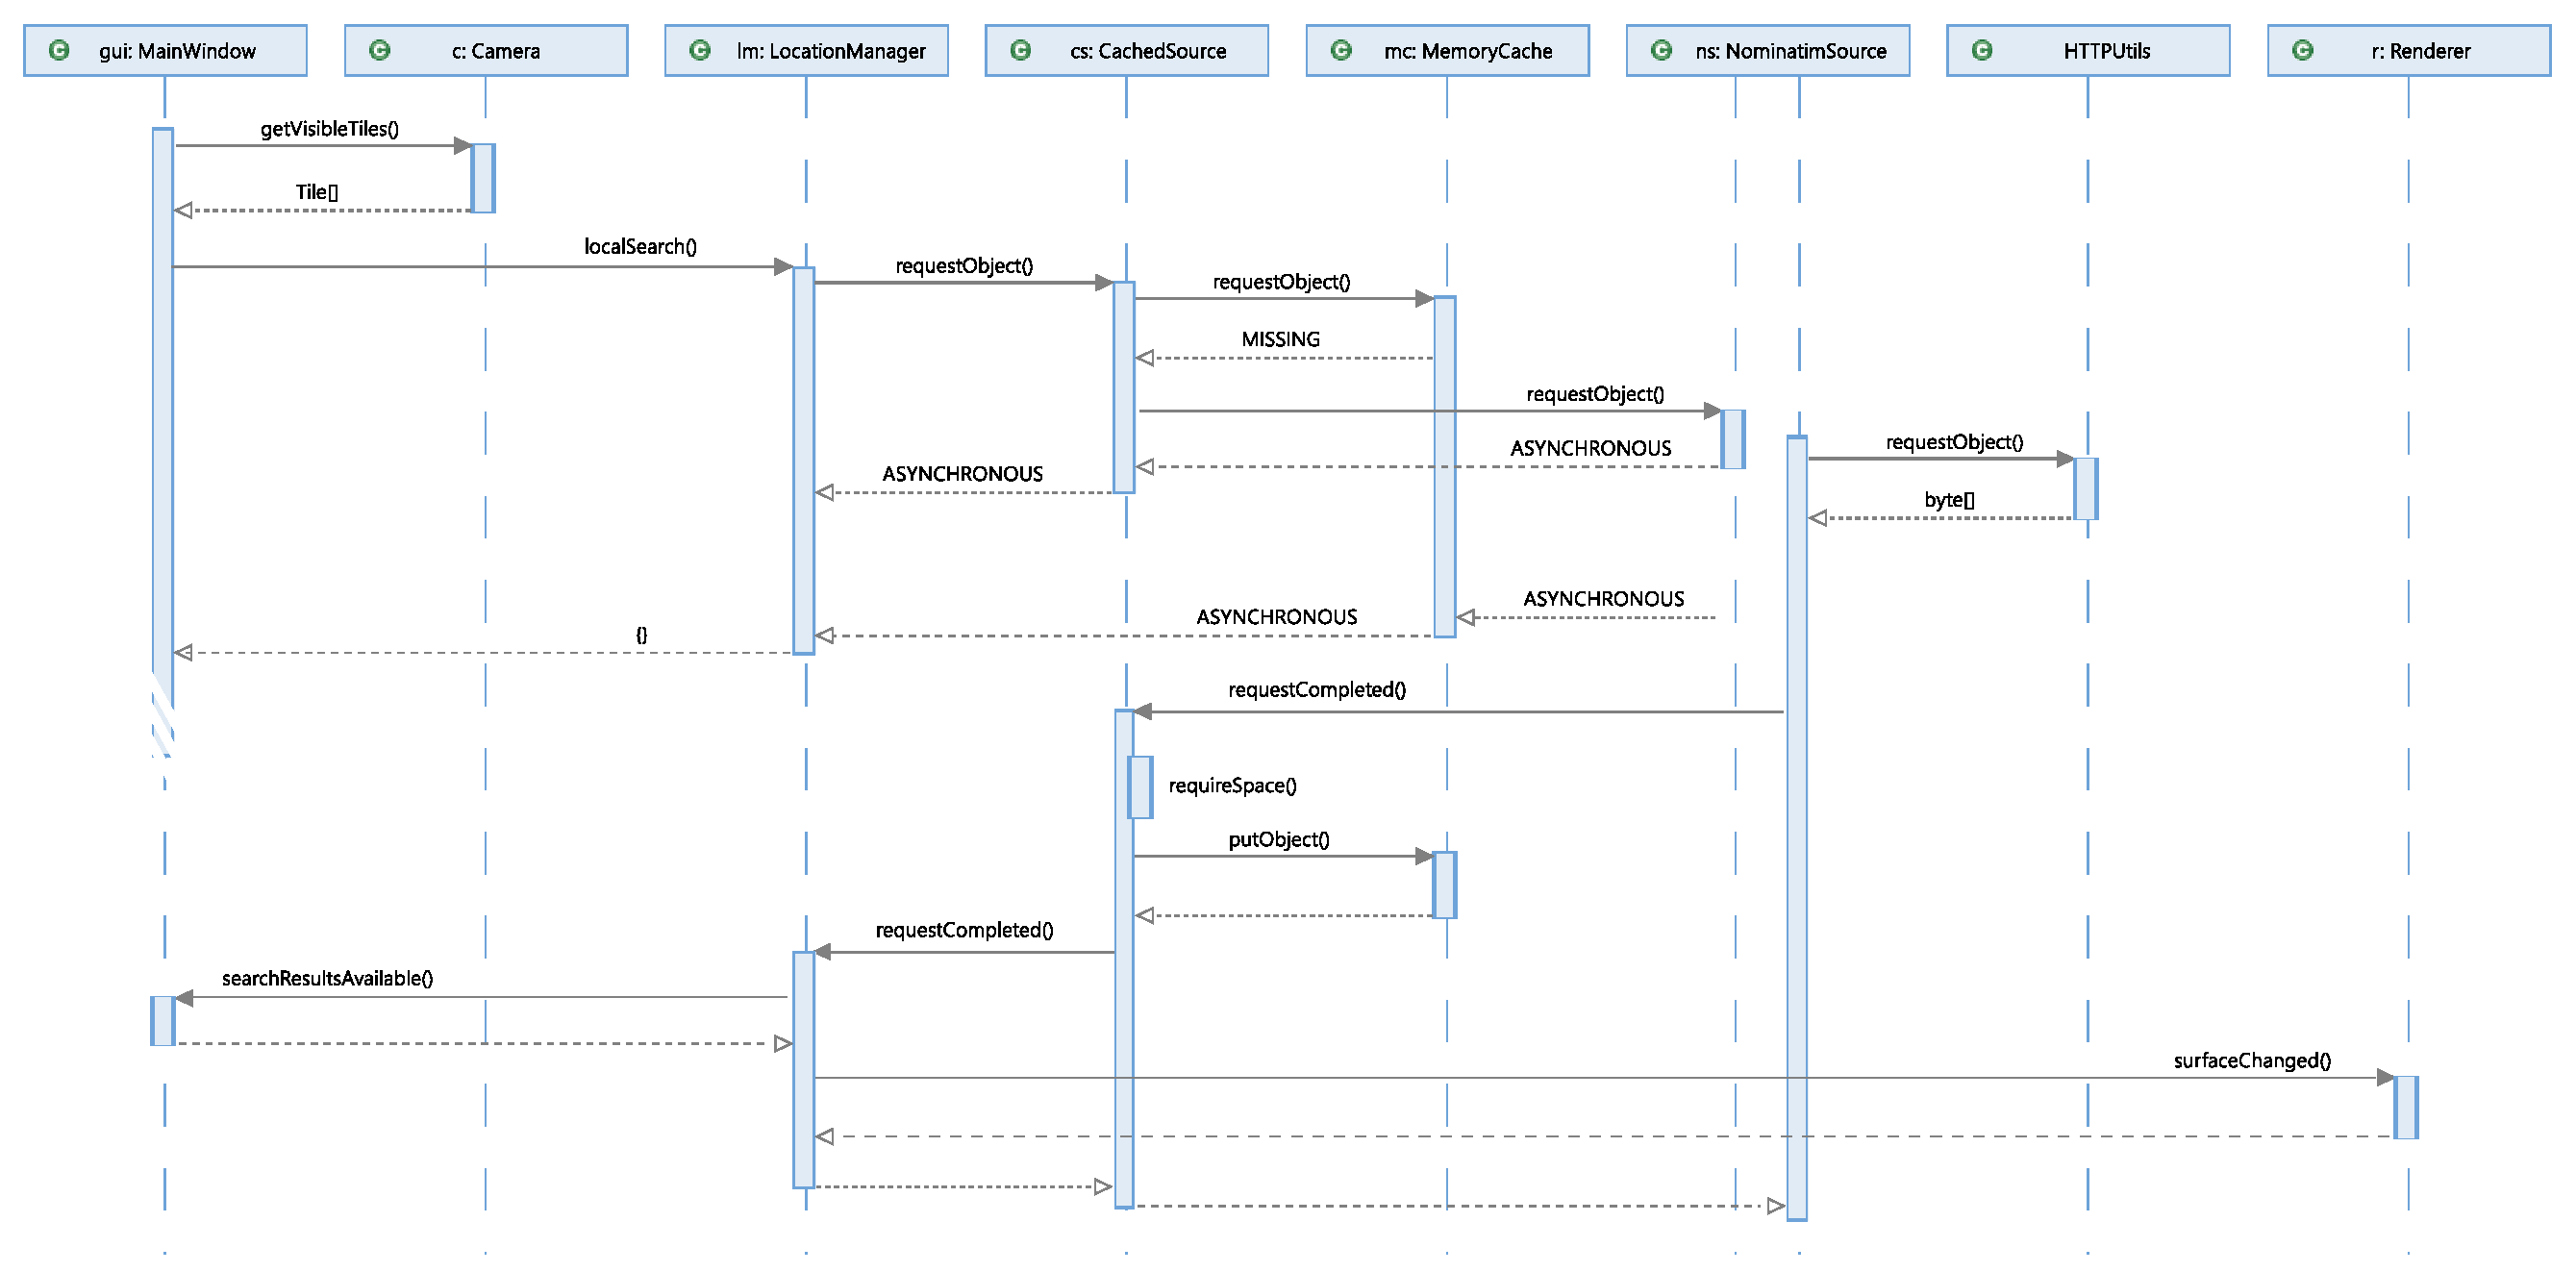
\includegraphics[scale=0.28]{sequenz-search.eps}
\caption{Lokale Suche nach einem Begriff}
\end{center}
\end{figure}

\begin{itemize}
\item Die GUI übergibt dem \textit{LocationManager} einen Suchbegriff und die sichtbaren Kacheln, die er von der Kamera erhalten hat.
\item Dieser fordert von seinem \textit{RequestDistributor} die Suchergebnisse zu dieser Anfrage an, der wegen des Fehlens des Ergebnisses in seinem \textit{MemoryCache} bei der \textit{NominatimSource} eine Anfrage startet. 
\item Da eine Anfrage über das Internet zeitaufwändig ist, kehrt sie und damit der \textit{RequestDistributor} mit der Notiz zurück, dass eine asynchrone Antwort folgt. Die GUI erhält daher zuerst ein leeres Ergebnis.
\item Wurde die Anfrage beantwortet, benachrichtigt die \textit{NominatimSource} den \textit{RequestDistributor}, der die Antwort in seinen \textit{MemoryCache} legt und seinerseits den \textit{LocationManager} benachrichtigt.
\item Der GUI, die ein \textit{LocationListener} ist, wird mitgeteilt, dass die Suchergebnisse jetzt verfügbar sind.
\end{itemize}
\newpage


\section{Laden einer lokal noch nicht vorhandenen Kachel}

In diesem Sequenzdiagramm wird dargestellt, wie die Anfrage nach einer Texturkachel über die verschiedenen Cacheebenen propagiert und schließlich asynchron beantwortet wird.\\[3mm]
Eine größere Version des Diagramms findet sich im Anhang (\textref Abbildung 9.2).

\vspace*{5mm}
\begin{figure}[h]
\begin{center}
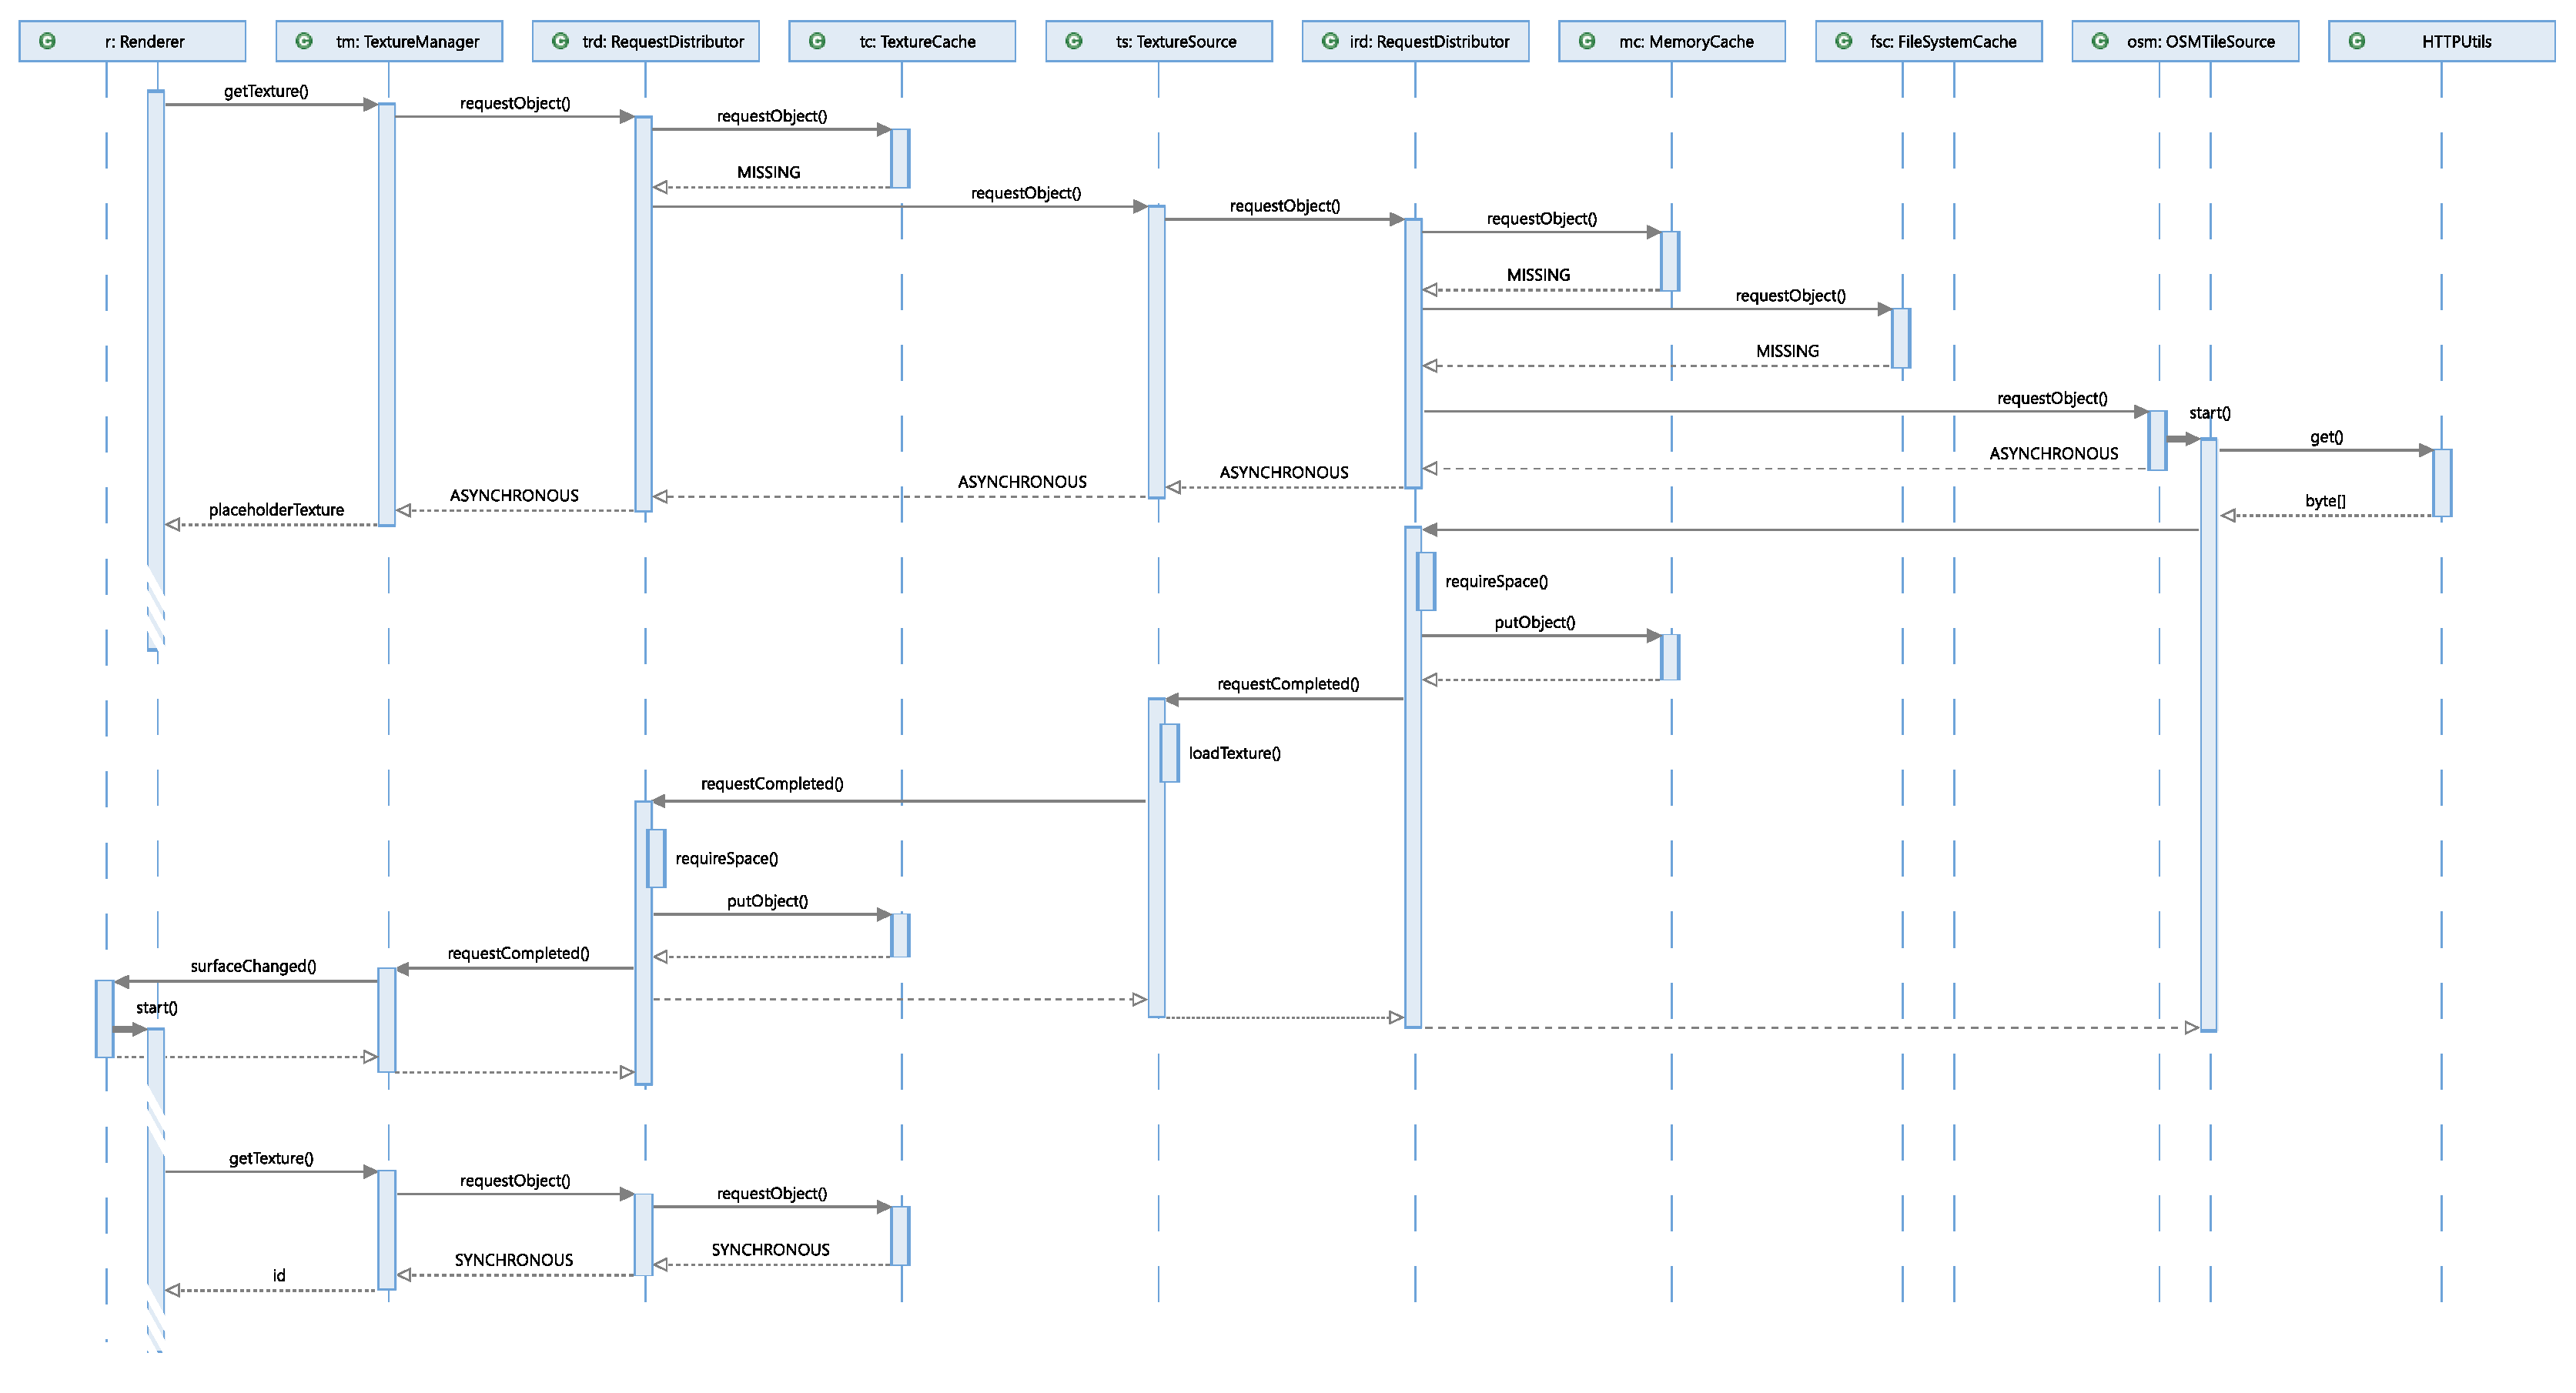
\includegraphics[scale=0.28]{sequenz-osmtile.eps}
\caption{Laden einer lokal noch nicht vorhandenen Kachel}
\end{center}
\end{figure}

\begin{itemize}
\item Der \textit{Renderer} fragt den \textit{TextureManager} nach der Textur für eine Kachel.
\item Dieser fordert von seinem \textit{RequestDistributor} die Ergebnisse zu dieser Anfrage an.
\item Im Beispiel ist die Textur noch nicht im \textit{TextureCache} vorhanden. Deswegen leitet der \textit{RequestDistributor} die Anfrage an die \textit{TextureSource} weiter.
\item Die \textit{TextureSource} fordert den \textit{RequestDistributor} für die Bilddateien auf, die Kachel zu beschaffen.
\item Da sich die Textur in unserem Beispiel weder im \textit{Memory-} noch im \textit{FileSystemCache} befindet, wird die Textur über die \textit{OSMTileSource} geladen, die darauf hinweist, dass die Antwort asynchron erfolgt und ohne Ergebnis zurückkehrt.
\item Der \textit{TextureManager} gibt ersatzweise die Platzhaltertextur zurück.
\item Ist das Kachelbild geladen, wird es vom Bild-\textit{RequestDistributor} in seinem \textit{MemoryCache} abgelegt.
\item Der \textit{RequestDistributor} benachrichtigt die \textit{TextureSource} über die vorhandene Bilddatei, die jetzt die Textur in OpenGL lädt und an ihren \textit{RequestDistributor} weiterleitet.
\item Diese informiert \textit{TextureManager}, der dem \textit{Renderer} mitteilt, dass sich die Darstellung der Kachel nun geändert hat.
\item Der \textit{Renderer} beginnt daraufhin einen neuen Frame mit der korrekten Textur zu zeichnen.
\end{itemize}


\newpage

\section{Aktivieren des Höhenprofils; Nachladen benötigter SRTM-Daten}
Im diesem Sequenzdiagramm wird sichtbar, wie nach Aktivierung des Höhenprofils über den \textit{HeightMapManager} SRTM-Daten nachgeladen werden.
Eine größere Version des Diagramms findet sich im Anhang (\textref Abbildung 9.3).

\vspace*{5mm}
\begin{figure}[h]
\begin{center}
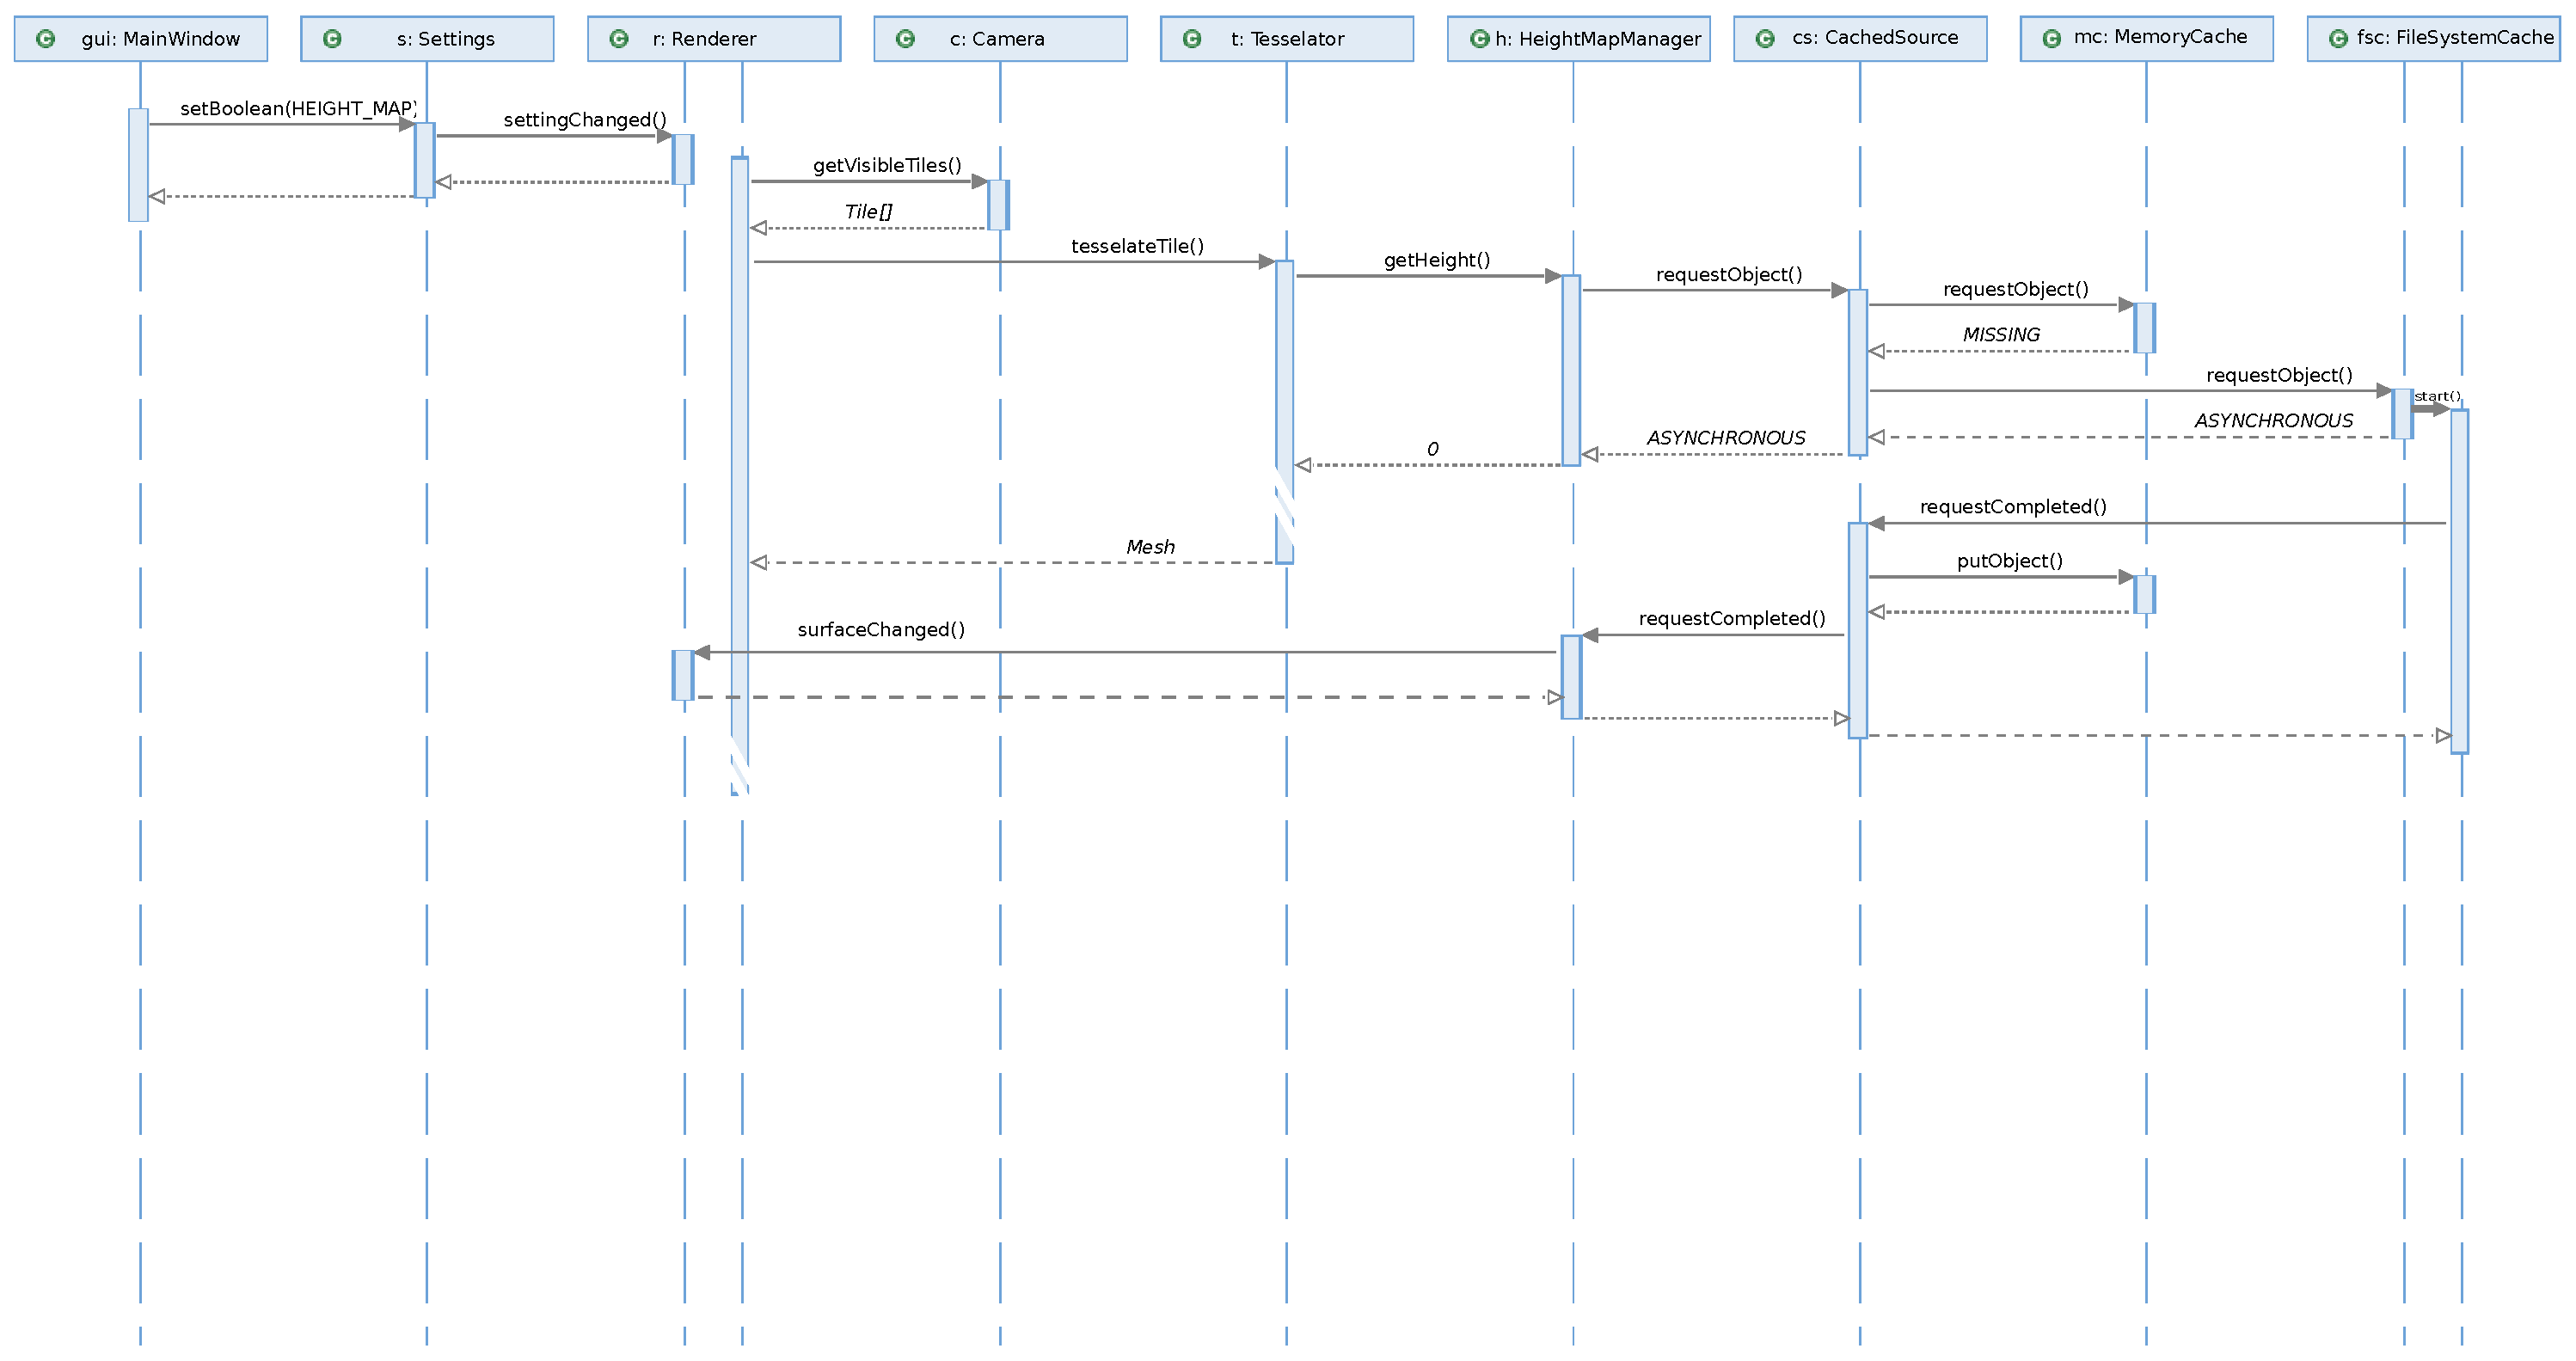
\includegraphics[scale=0.28]{sequenz-height.eps}
\caption{Aktivieren des Höhenprofils; Nachladen benötigter SRTM-Daten}
\end{center}
\end{figure}

\begin{itemize}
\item Im \textit{MainWindow} wurde die Höhenprofil-Einstellung aktiviert. Dies verändert eine Eigenschaft in den \textit{Settings}, welche den \textit{Renderer} über die Änderung benachrichtigt.
\item Dieser beginnt asynchron, eienn neuen Frame zu zeichnen, wozu er bei der \textit{Camera} die sichtbaren Kacheln anfordert und von seinem \textit{Tesselator} generieren lässt.
\item Der \textit{Tesselator} fordert beim \textit{HeightMapManager} die Höhe der einzelnen Punkte an.
\item Dieser versucht, die SRTM-Kachel, die die Höheninformation trägt. bei seinem SRTM-\textit{RequestDistributor} anzufordern.
\item Im Beispiel liegt diese Kachel zwar nicht im \textit{Memory}-, aber im \textit{FileSystemCache}. Da das Laden von der Festplatte etwas Zeit in Anspruch nehmen kann, kehrt die Methode mit der Notiz zurück, dass eine asynchrone Antwort folgt.
\item Da die Höhenkachel im Moment nicht zur Verfügung steht, gibt der \textit{HeightMapManager} 0 (Normalnull) als Höhe für den Punkt zurück.
\item Sobald die verspätete Antwort des \textit{FileSystemCaches} eintrifft, wird der \textit{Renderer} aufgefordert ein neues Bild zu zeichnen.
\item Er fordert nun die selben Höhendaten an, die aber aus dem \textit{MemoryCache} des \textit{HeightMapManagers} beantwortet werden können.
\end{itemize}

\newpage

\section*{Semantik der Diagramme}
\begin{itemize}
\item Senkrechte gestrichelte Linien enthalten sequentielle Aufrufe (\textit{Lebenslinien}). Gibt es zu einem Objekt oder einer Klasse mehrere solcher Linien, bedeutet dies, dass Aufrufe parallel in verschiedenen Threads ausgeführt werden.
\item Threads werden mit der asynchronen Nachricht \texttt{start()} angestoßen. Sie können beispielsweise mit einem \textit{ExecutorService} implementiert werden, der einzelne asynchrone Aktionen ausführen kann.
\item Blau-weiß diagonal unterbrochene Lebenslinien zeigen an, dass an dieser Stelle weiter Aufrufe vor Rückkehr der Funktion stattfinden, die aber für den Ausschnitt des Sequenzdiagramms keine Rolle spielen.
\end{itemize}


\chapter{Design Patterns}

\section{Systemarchitektur: Model-View-Controller}

Das \textit{Model-View-Controller Pattern} ist das Architekturmuster, nach dem die grundlegende Architektur des Programms strukturiert wurde.\\
\begin{figure}[ht]
\begin{centering}
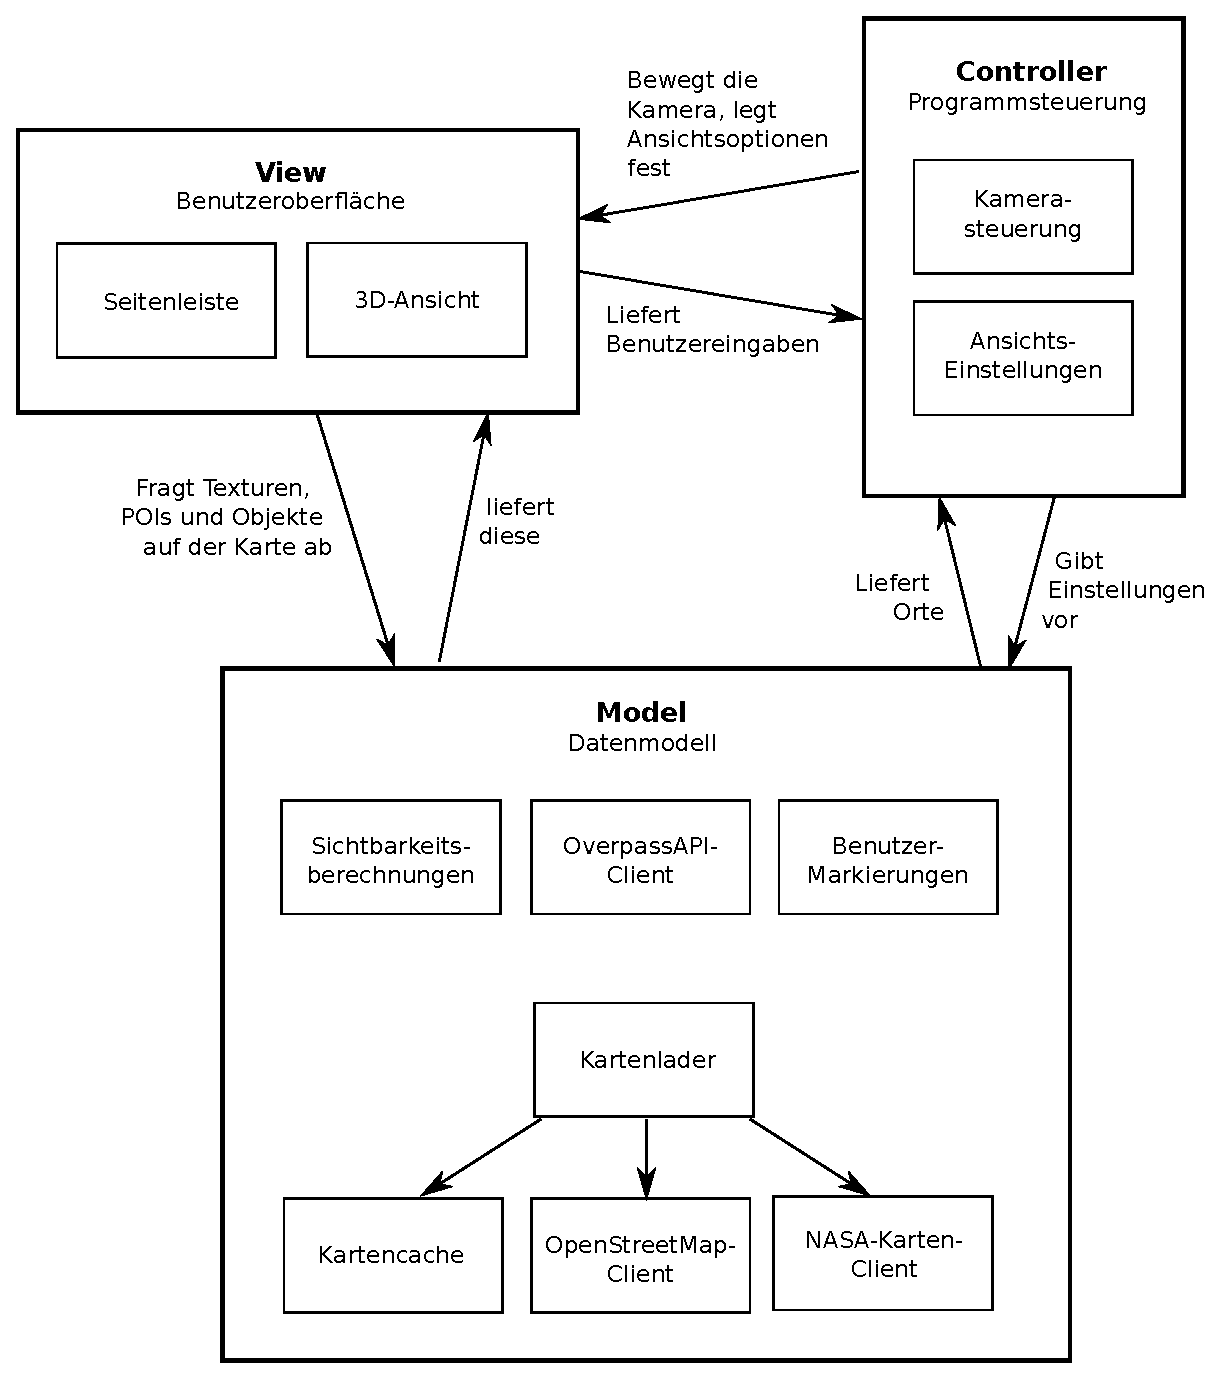
\includegraphics[scale=0.5]{ModelViewController.eps}
\caption{Das Model-View-Controller Pattern}
\end{centering}
\end{figure}

Es teilt die Funktionalität der Komponenten in Datenmodell (\textit{Model}), Präsentation (\textit{View}) und Steuerung (\textit{Controller}) ein. Das Datenmodell beinhaltet dabei die zugrundeliegende Datenverwaltung und  Berechnungsmodelle, die Präsentation ist für die Schnittstelle zum Nutzer verantwortlich, und der Controller nimmt Eingaben entgegen und steuert die View bzw. Views.

\newpage

\section{Weitere verwendete Entwurfsmuster}

\subsection{Adapter Pattern}
Das \textit{Adapter Pattern} ist ein Strukturmuster. \\
Es dient zur Übersetzung einer Schnittstelle in eine andere. \\ Dieses Pattern findet Anwendung bei den \textit{Mouse- und Key"-listenern}, welche in der Benutzeroberfläche implementiert werden. \\ Ziel ist es den Quellcode übersichtlich zu halten. Aus diesem Grund werden nur die benötigten Methoden der Listener überschrieben. Alle nicht erforderlichen Methoden werden ignoriert.

\subsection{Chain of Responsibility Pattern}
Das \textit{Chain of Responsibility Pattern} (bzw. Zuständigkeitskette) ist ein Verhaltensmuster. \\
Hierbei werden mehrere Objekte hintereinander verkettet um gemeinsam eine eingehende Anfrage bearbeiten zu können. Dafür wird eine Anfrage entlang der Kette durchgereicht, bis ein Objekt die Anfrage beantworten kann. \\ Es findet Anwendung beim Speichermanagement. Eine Anfrage für eine benötigte Ressource wird immer an den \textit{RequestDistributor} gestellt. Die Anfrage wird entsprechend der Kette (\textref Sequenzdiagramm 6.2) durchgereicht bis sie bearbeitet werden kann. \\ Ziel ist die Entkopplung des Auslösers einer Anfrage mit seinem Empfänger.

\subsection{Data Transfer Object}
Das \textit{Data Transfer Object} ist ein Muster für eine objektrelationale Abbildung. \\
Hierbei werden mehrere Daten gebündelt als ein Objekt übertragen. \\ Es findet Anwendung bei Suchergebnissen und der Anfrage nach POIs. Alle Datensätze werden dann gebündelt übergeben und nicht jede Information seperat. \\ Ziel ist es die Daten zu strukturieren bzw. vollständig gruppierte Information zu einer Anfrage zu erhalten.

\subsection{Iterator Pattern}
Das \textit{Iterator Pattern} ist ein Verhaltensmuster.\\ Hierbei wird die verwendete Datenstruktur elementweise durchlaufen, ohne deren interne Anordnung preiszugeben.\\ Es findet Anwendung bei der Verdrängungsstrategie. Es werden die verschiedenen Caches elementweise durchlaufen um die entsprechenden Einträge zu verdrängen.\\
Ziel ist es die eingesetzten Datenstrukturen effizient zu durchsuchen.

\subsection{Mediator Pattern}
Das \textit{Mediator Pattern} ist ein Verhaltensmuster. \\ Hierbei fungiert der Vermittler als Kommunikationsschnittstelle zwischen Objekten in einem komplexen System.\\ Es findet mehrfache Anwendung im gesamten Programm, wie beispielsweise beim Speichermanagement, beim Rendering, usw. \\ Ziel ist lockere Kopplung. Es sollen nicht alle Objekt voneinander Kenntnis besitzen.



\subsection{Observer Pattern}
Das \textit{Observer Pattern} ist ein Verhaltensmuster. \\ Hierbei wird eine Info bei durchgeführten Änderungen am Objekt an alle abhängigen Komponenten weitergegeben. \\ Es findet beispielsweise Anwendung beim \textit{SettingsListener}, \textit{CameraListener}, \textit{SurfaceListener} usw. \\ 
Ziel ist lose Kopplung und zudem werden die abhängigen Objekte automatisch über Änderungen in Kenntnis gesetzt.

\subsection{Singleton Pattern}
Das \textit{Singleton Pattern} ist ein Erzeugungsmuster. \\ Hierbei wird sichergestellt, dass genau eine einzige Instanz eines Objekts existiert. \\ Es findet Anwendung bei den \textit{Settings}, von der nur eine Instanz existieren darf. \\ Ziel ist eine sichergestellte Zugriffskontrolle auf das Objekt.




\chapter{Qualitätsmerkmale}
\section{Entwurfsqualität}
Bei der Qualitätsbewertung des Entwurfs beziehen wir uns auf \textit{Robert Cecil Martins} Merkmalsdefinitionen \footnote{Robert Cecil Martin (2002). Agile Software Development: Principles, Patterns and Practices. Pearson Education.} die im Folgenden erläutert werden.

\subsection*{Anzahl an Klassen und Interfaces}
Die Anzahl aller Klassen inklusive abstrakter Klassen (sowie Interfaces) im gesamten Paket. Sie dient als aussagekräftiger Indikator für die Erweiterbarkeit eines Pakets.

\subsection*{Afferente Kopplung}
Die Abhängigkeit anderer Pakete von einem Paket ist ein Maß für dessen Verantwortlichkeiten und Einfluss.

\subsection*{Efferente Kopplung}
Die Abhängigkeit eines Pakets von anderen Paketen ist ein Maß für seine Unselbstständigkeit.

\subsection*{Abstraktheit}
Der Anteil abstrakter Klassen und Interfaces an allen Klassen im Paket ist ein Indikator für den Abstraktionsgrad eines Pakets.

\subsection*{Stabilität}
Das Verhältnis von afferenter Kopplung zur gesamten Kopplung gibt Auskunft über die Resilienz gegenüber Änderungen in einem Pakets.

\subsection*{Balance von Abstraktion und Abhängigkeit}
Der Abstraktionsgrad der Klassen sollte in etwa deren Unabhängigkeit von anderen Klassen entsprechen. Bei Erfüllung der Anforderung spricht man von optimaler Balance.

\subsection*{Kohäsion}
Als Ergänzung zu Martins Definitionen, welche sich nur auf das Zusammenspiel zwischen den Paketen bezieht, wird zudem die Kohäsion berücksichtigt.\\

Kohäsion ist der Versuch, zusammenhängende Programmstrukturen in einer Klasse zusammenzuführen, um z.B. nachträgliche Änderungen auf lokale Anpassungen des Codes zu beschränken.


\section{Gütekriterien nach ISO/IEC 9126}
\subsection*{Funktionalität}
Funktionalität beinhaltet Angemessenheit, Richtigkeit, Interoperabilität, Ordnungsmäßigkeit und Sicherheit.

\subsection*{Zuverlässigkeit}
Eine Menge von Merkmalen, die sich auf die Fähigkeit einer Software/eines Systems beziehen, ihr/sein Leistungsniveau unter festgelegten Bedingungen über einen festgelegten Zeitraum oder über eine festgelegte Anzahl von Transaktionen zu bewahren. [ISO 9126]

\subsection*{Benutzbarkeit}
Die Fähigkeit eines Softwareprodukts, unter spezifizierten Bedingungen für einen Benutzer verständlich, erlernbar, anwendbar und attraktiv zu sein. [ISO 9126]

\subsection*{Effizienz}
Die Fähigkeit eines Softwareprodukts, unter festgelegten Bedingungen eine angemessene Leistung zu erbringen, bezogen auf den Umfang der eingesetzten Betriebsmittel. [ISO 9126]

\subsection*{Änderbarkeit}
Mit Änderbarkeit bezeichnet man den Aufwand, der zur Durchführung bestimmter Änderungen notwendig ist. Änderungen können Korrekturen, Verbesserungen oder Anpassungen an Änderungen der Umgebung, der Anforderungen und der funktionalen Spezifikation einschließen. [ISO 9126]

\subsection*{Portabilität}
Portabilität oder Übertragbarkeit ist die Eignung einer Software, von einer Umgebung in eine andere übertragen zu werden. Diese Umgebung kann die organisatorische Umgebung, Hardware- oder Software-Umgebung einschließen. [ISO 9126]

\newpage
\pagestyle{empty}

\newgeometry{top=30mm, left=25mm, right=25mm, bottom=20mm}

\chapter{Anhang}
\centering
\thispagestyle{empty}
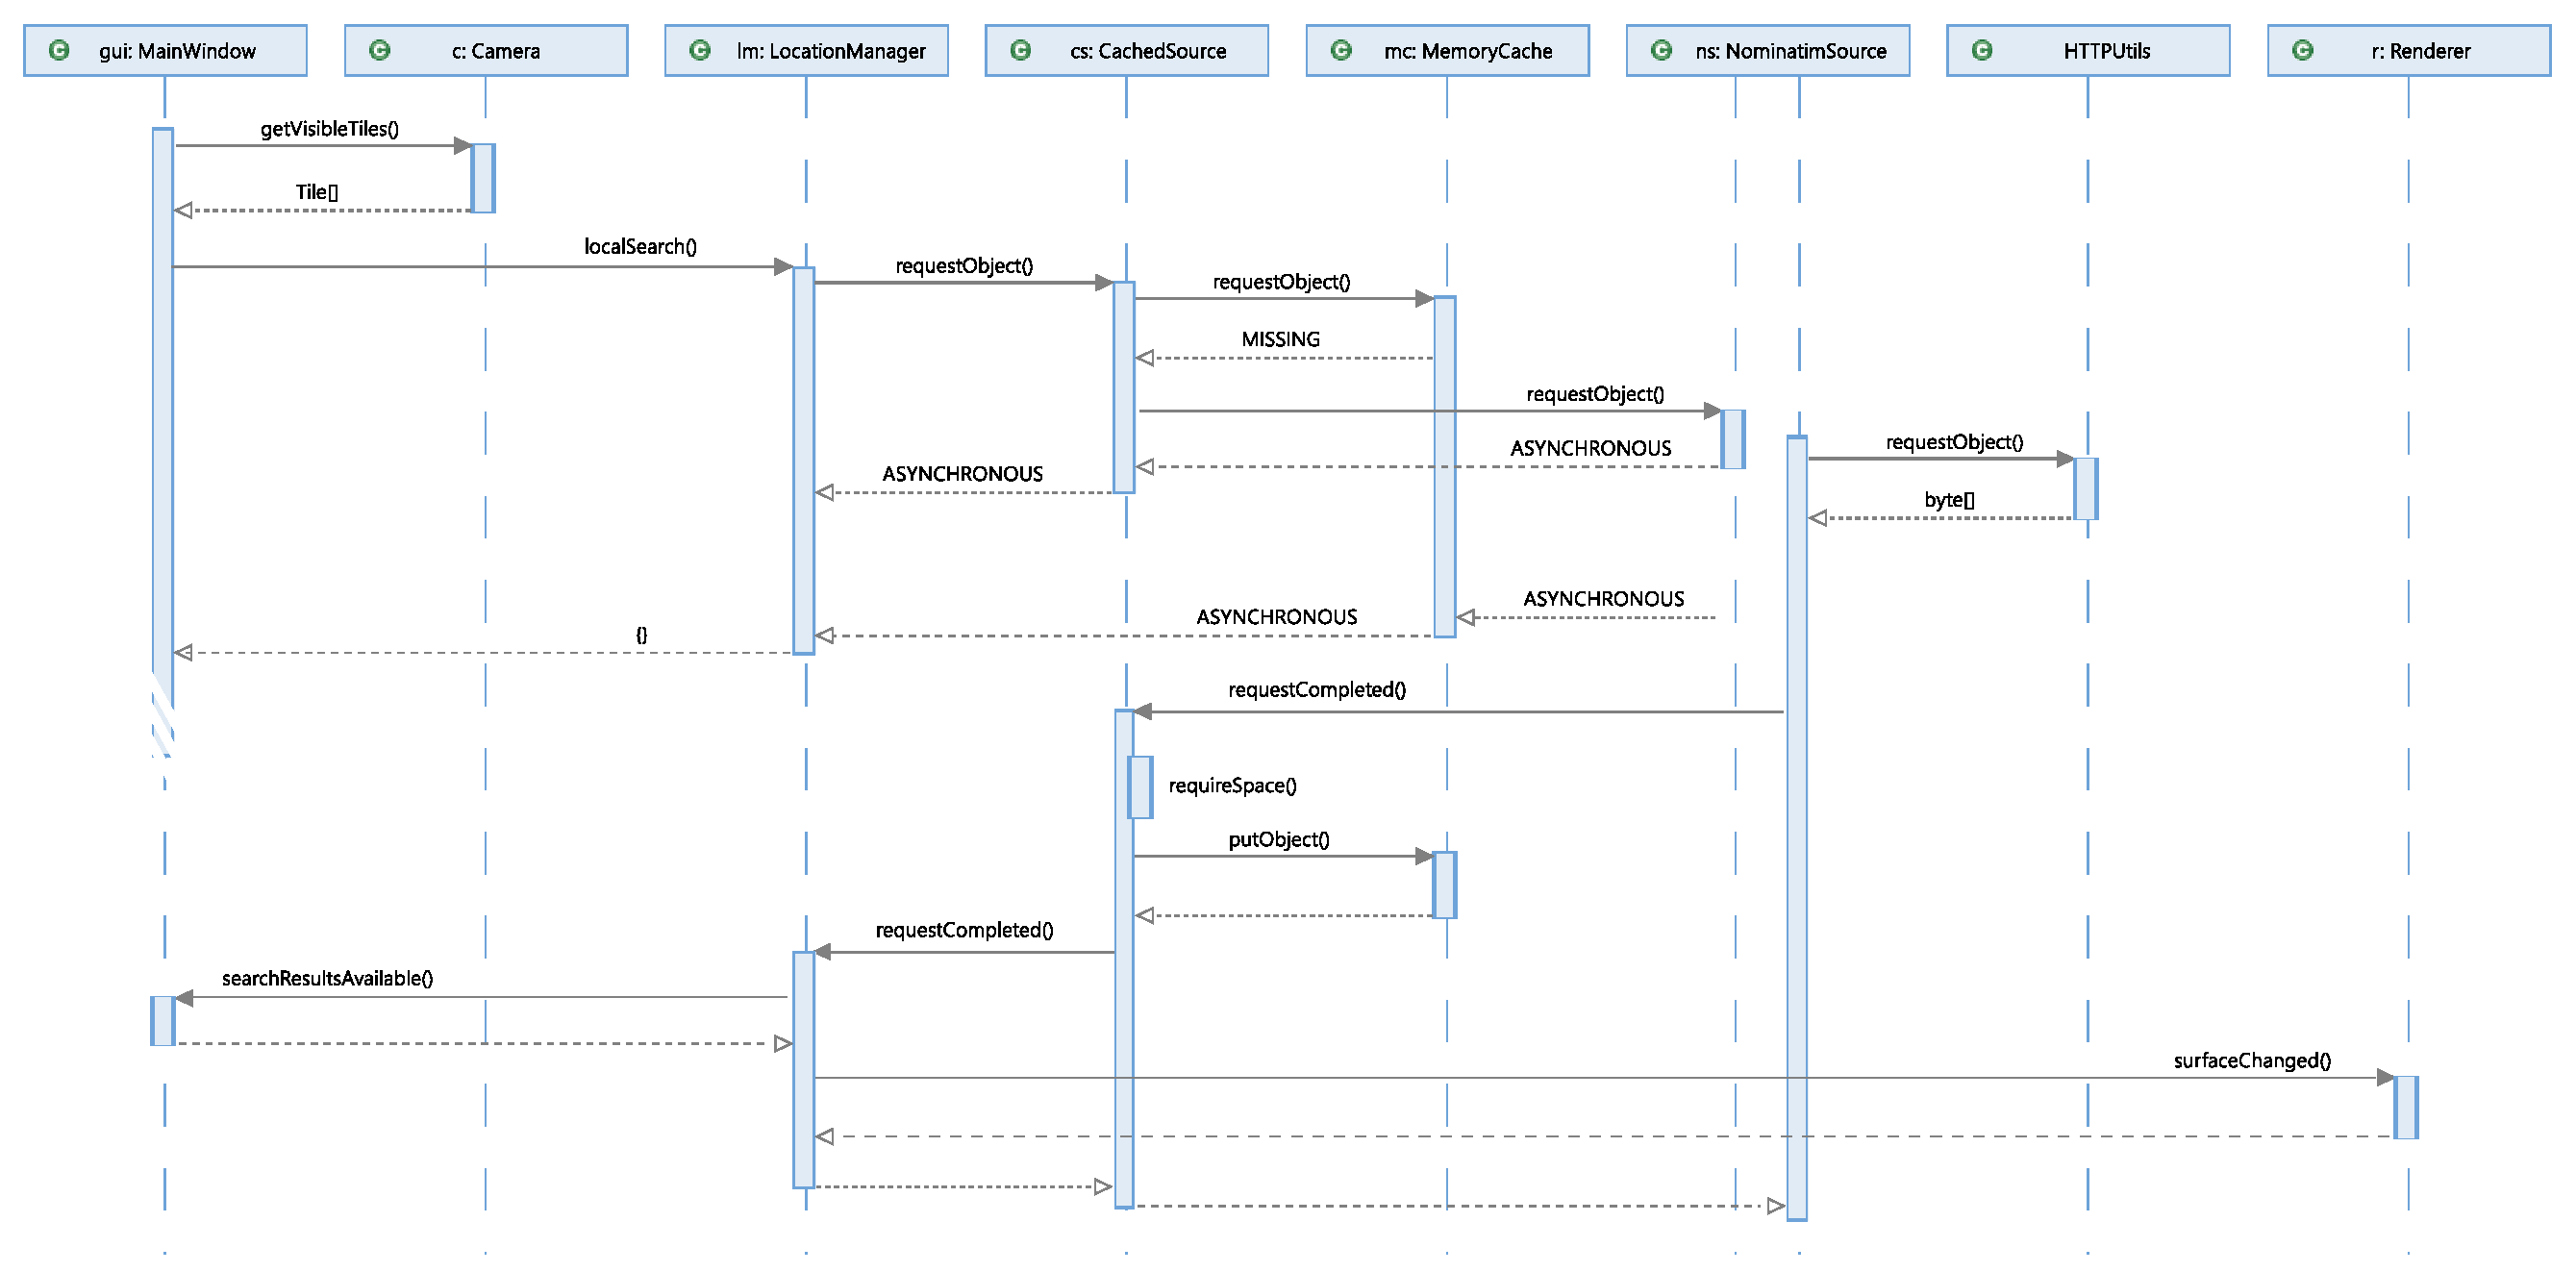
\includegraphics[scale=0.45,angle=90,origin=c]{sequenz-search.eps}
\hspace{5mm}
\begin{rotate}{90}
\textbf{Abbildung 9.1:} Sequenzdiagramm: Lokale Suche nach einem Begriff
\end{rotate}

\newpage
\newgeometry{top=20mm, left=15mm, right=15mm, bottom=20mm}
\thispagestyle{empty}
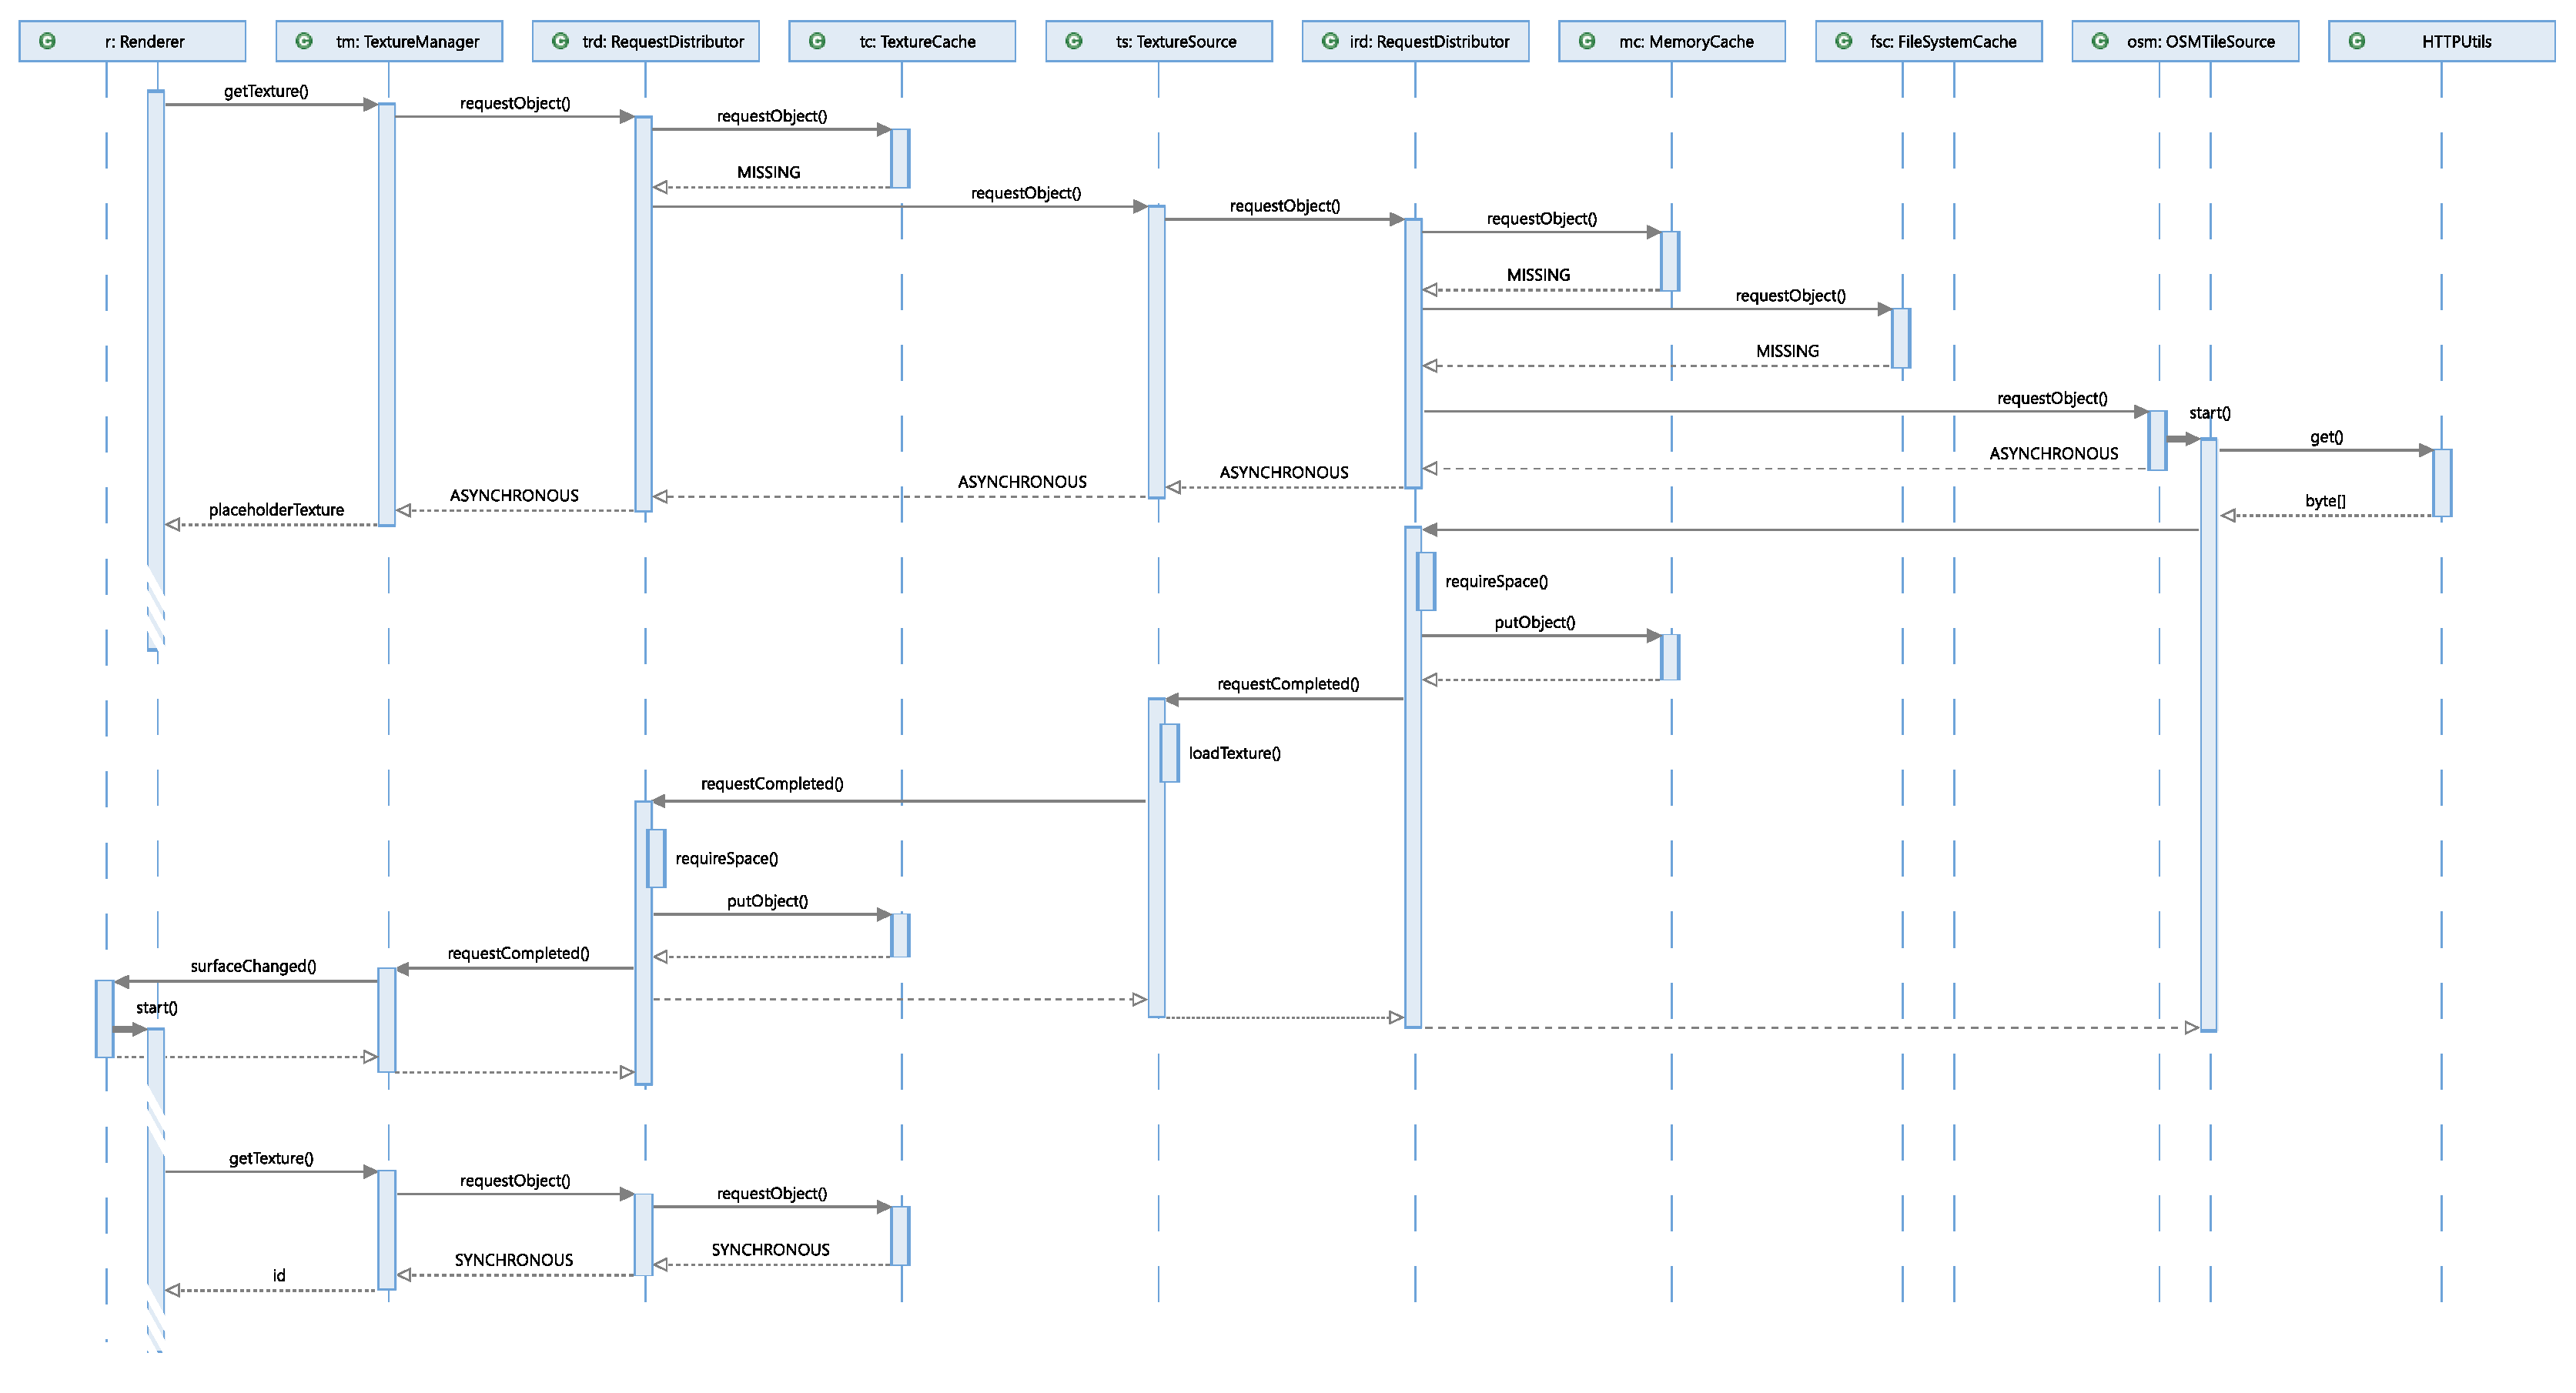
\includegraphics[scale=0.45,angle=90,origin=c]{sequenz-osmtile.eps}
\hspace{5mm}
\begin{rotate}{90}
\textbf{Abbildung 9.2:} Sequenzdiagramm: Laden einer lokal noch nicht vorhandenen Kachel
\end{rotate}

\newpage
\thispagestyle{empty}
\vspace*{1cm}
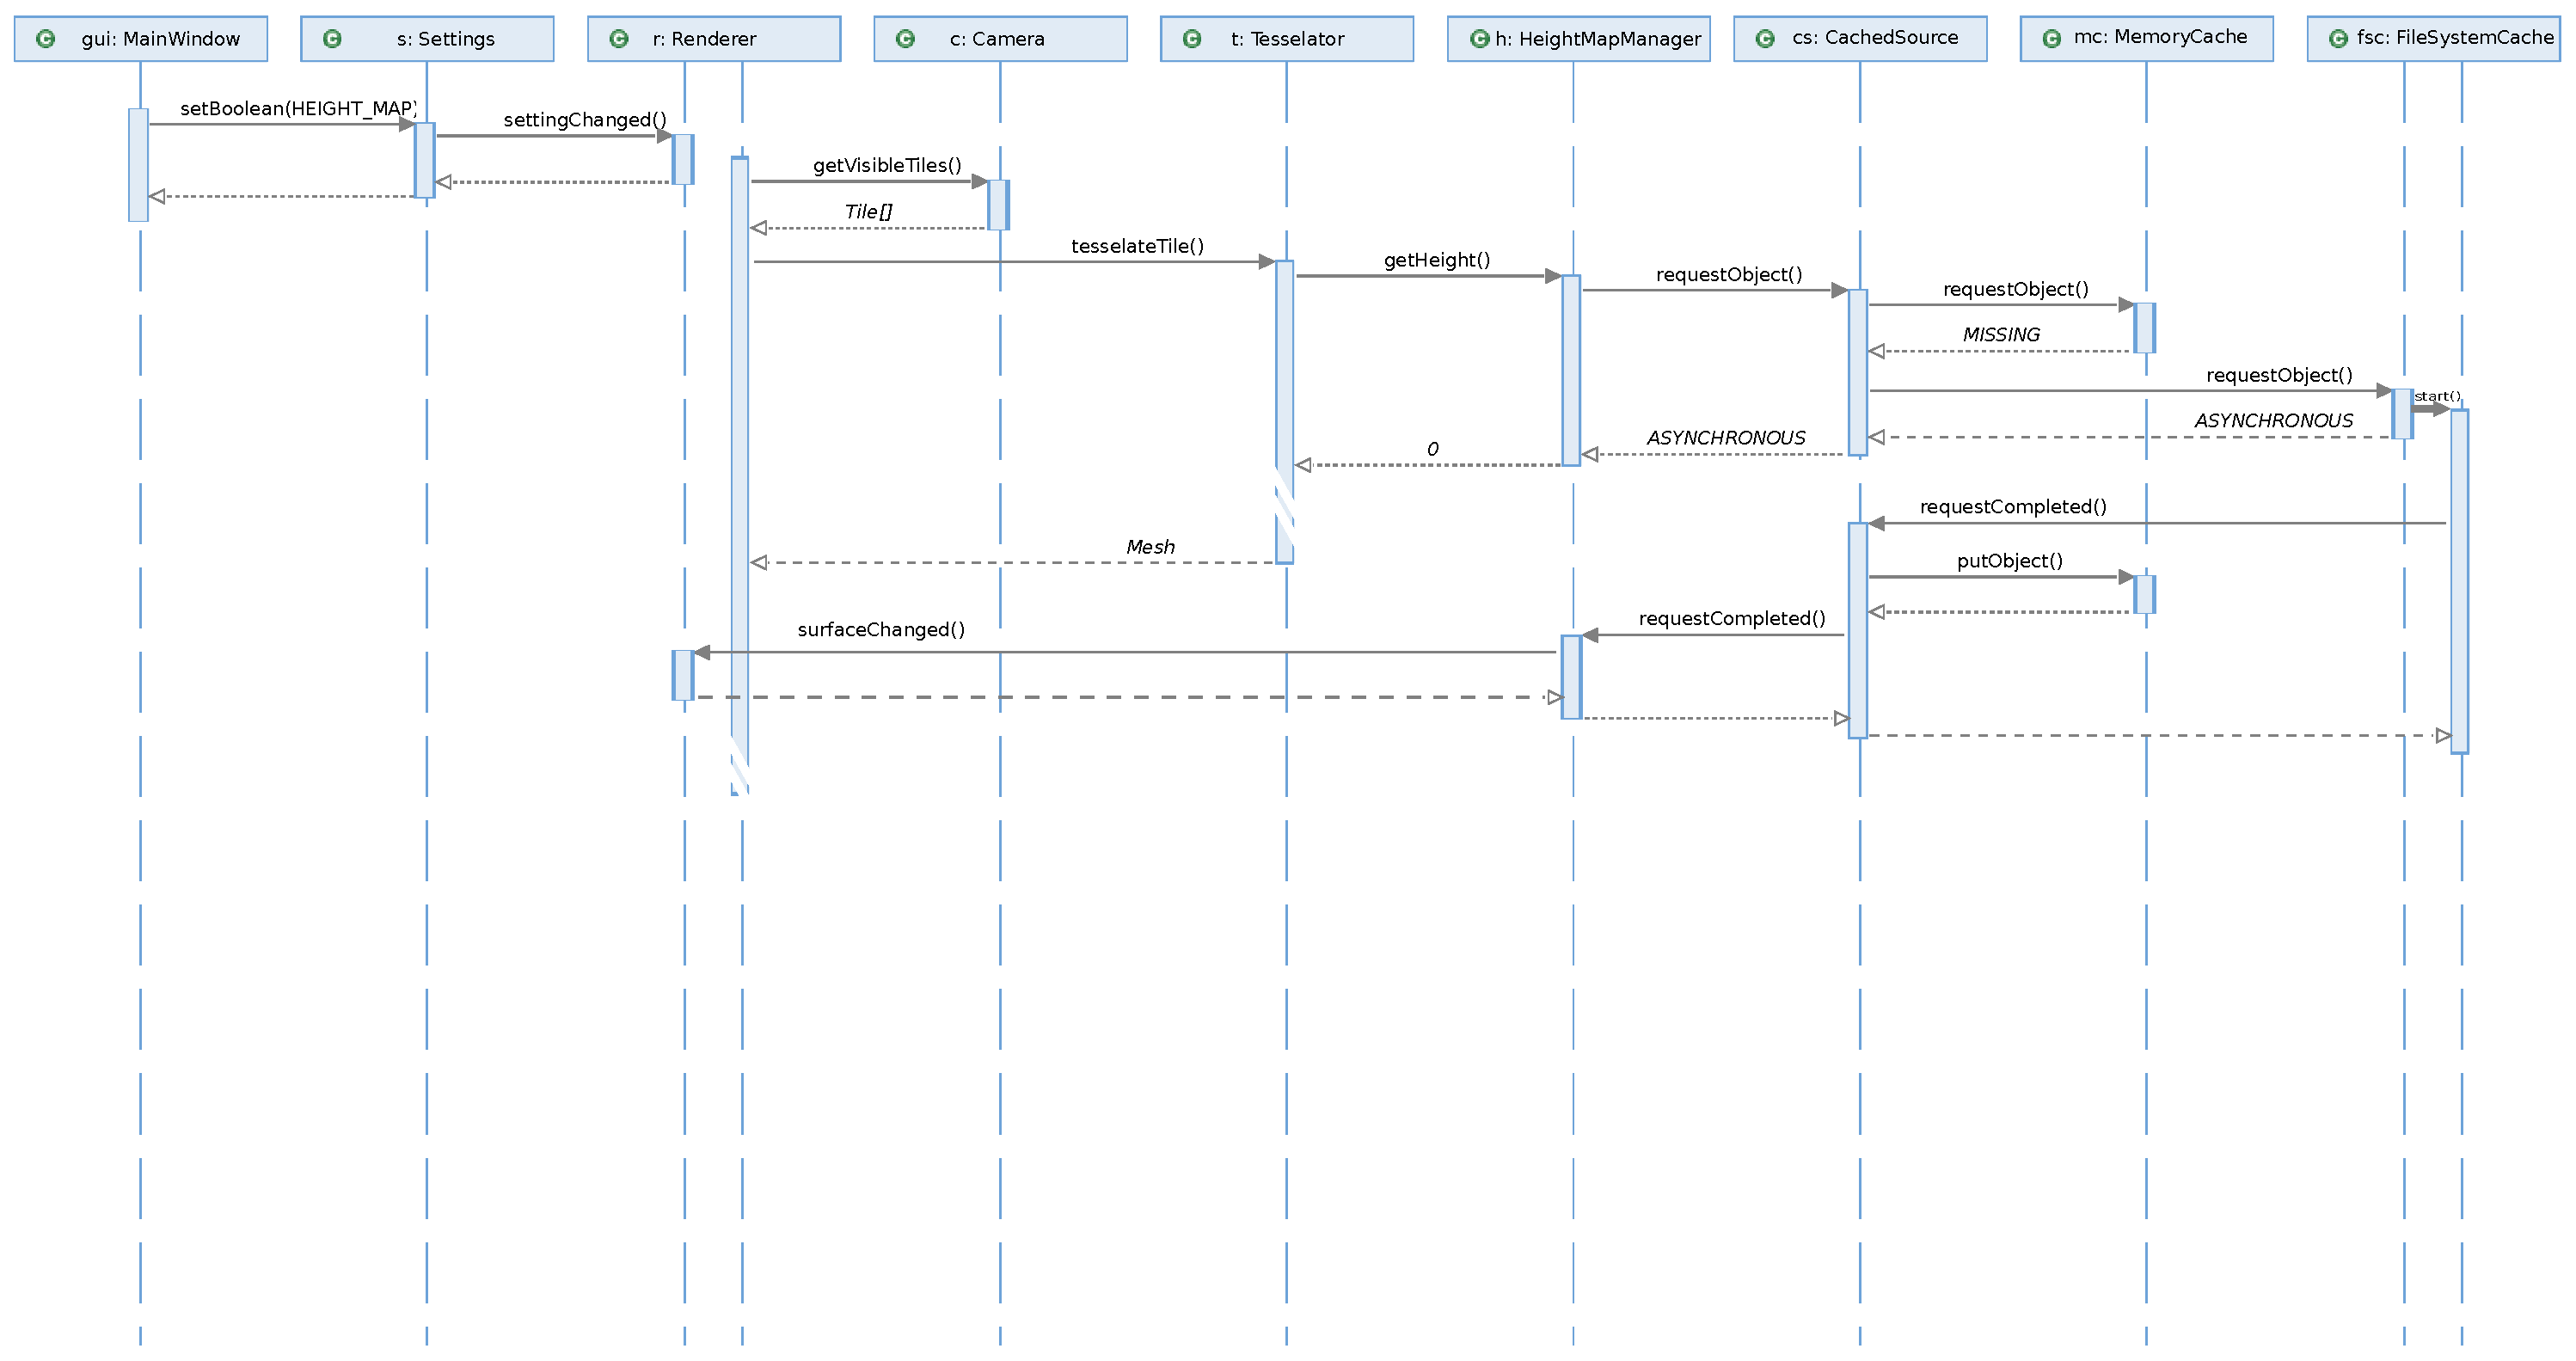
\includegraphics[scale=0.46,angle=90,origin=c]{sequenz-height.eps}
\hspace{5mm}
\begin{rotate}{90}
\textbf{Abbildung 9.3:} Sequenzdiagramm: Aktivieren des Höhenprofils; Laden benötigter SRTM-Daten
\end{rotate}

\newpage
\thispagestyle{empty}
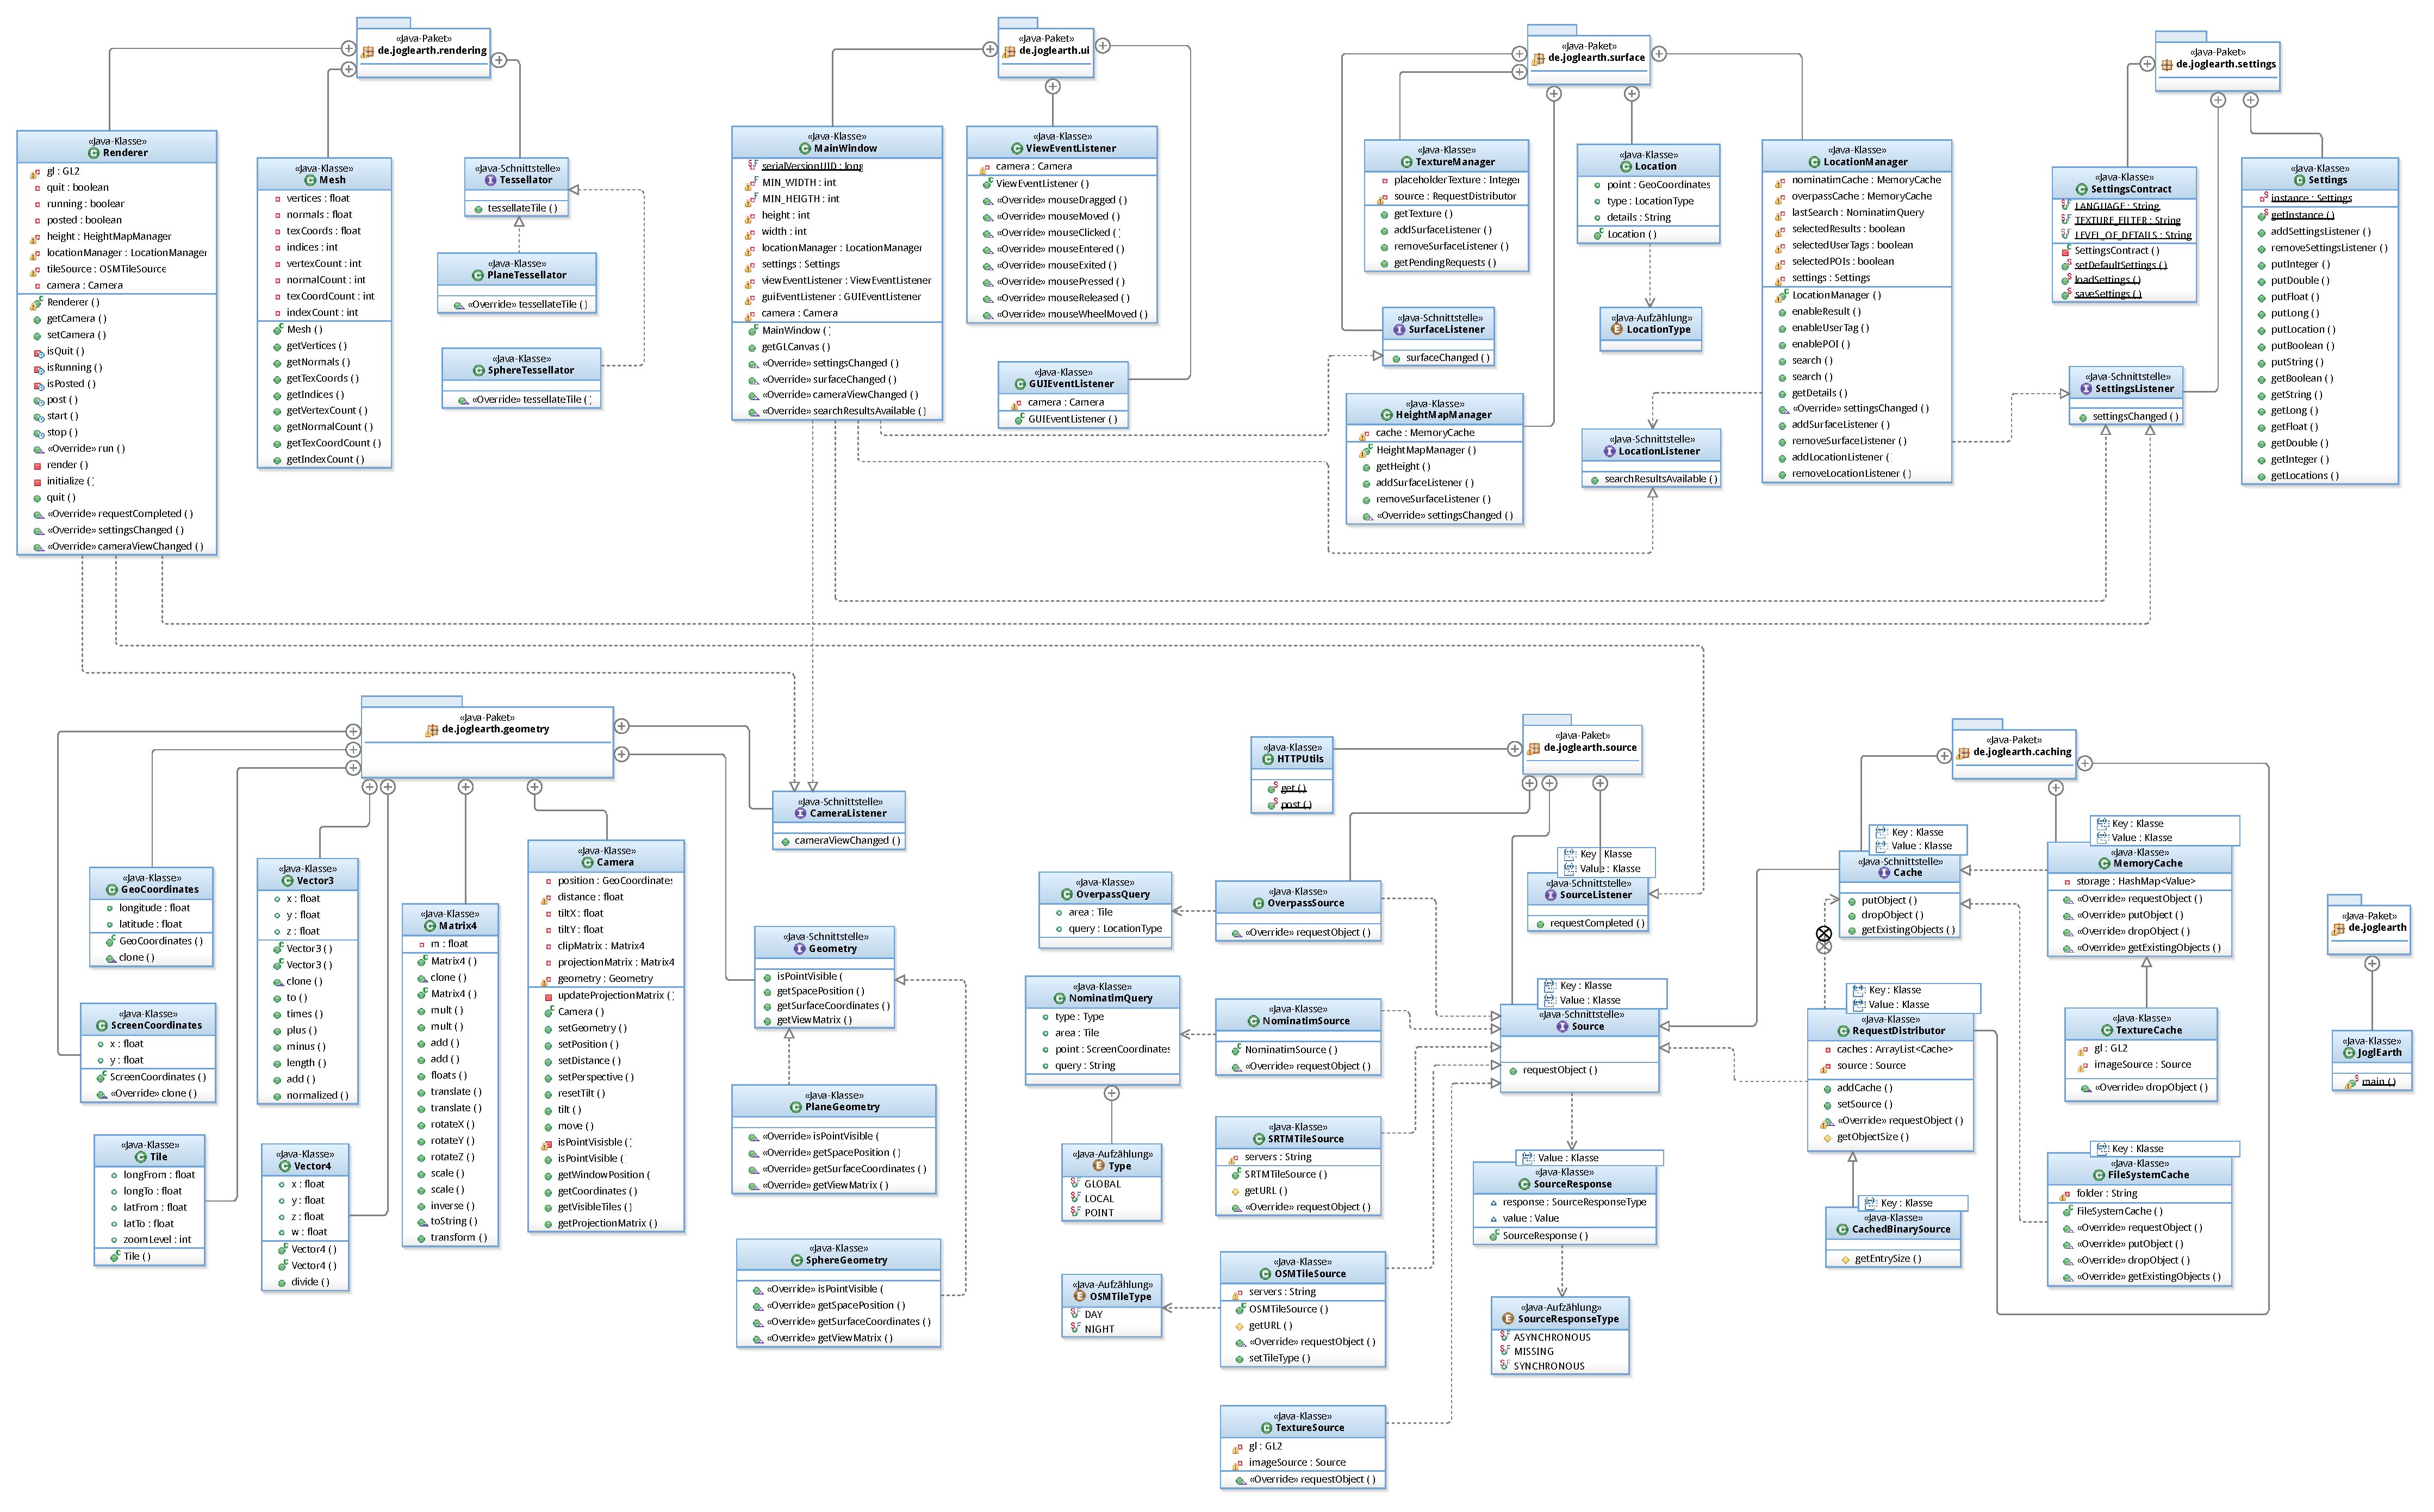
\includegraphics[scale=0.34,angle=90,origin=c]{JoglDiagramm_Main.eps}
\hspace{5mm}
\begin{rotate}{90}
\textbf{Abbildung 9.4:} Vollständiges Klassendiagramm
\end{rotate}


\restoregeometry

\end {document}